\chapter{PENGUJIAN DAN PEMBAHASAN}
\label{chap:pengujiandanpembahasan}

Dalam bab ini dijelaskan mengenai pengujian yang dilakukan berdasarkan hasil pelaksanaan pada bab \ref{chap:desainimplementasi}. Selain itu, juga dibahas dan dianalisa hasil dari pengujiannya. Melalui pengujian dan analisa mengenai hasil penelitian, diharapkan dapat menjadi acuan dalam pengambilan kesimpulan dari pelaksanaan tugas akhir ini.

% \section{Hasil Penelitian}
% \label{sec:hasilpenelitian}

% Hasil penelitian yang dimaksud disini merupakan hasil pelaksanaan dari tiap proses yang sudah dirancang sebelumnya pada tiap blok diagram metodologi dalam Bab \ref{chap:desainimplementasi}. Berikut ini adalah pembahasan mengenai tiap tahapannya.

% \subsection{Hasil Pengambilan Dataset}
% \label{subsec:hasilpengambilandataset}

% \subsection{Hasil Estimasi Pose}
% \label{subsec:hasilposeprediction}

% % \begin{figure}[!htb]
% %   \centering
% %   \begin{subfigure}{0.31\textwidth}
% %     \centering
% %     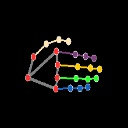
\includegraphics[width=\linewidth]{gambar/pose_prediction_next_slide.jpg}
% %     \caption{next slide}
% %     \label{fig:landmarknextslide} 
% %   \end{subfigure}
% %   \quad
% %   \begin{subfigure}{0.31\textwidth}
% %     \centering
% %     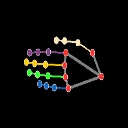
\includegraphics[width=\linewidth]{gambar/pose_prediction_previous_slide.jpg}
% %     \caption{previous slide}
% %     \label{fig:landmarkpreviousslide} 
% %   \end{subfigure}
% %   \quad
% %   \begin{subfigure}{0.31\textwidth}
% %     \centering
% %     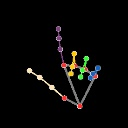
\includegraphics[width=\linewidth]{gambar/pose_prediction_pen_right.jpg}
% %     \caption{pen}
% %     \label{fig:landmarkpen}
% %   \end{subfigure}
% %   \quad
% %   \begin{subfigure}{0.31\textwidth}
% %     \centering
% %     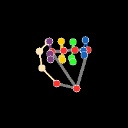
\includegraphics[width=\linewidth]{gambar/pose_prediction_erase.jpg}
% %     \caption{erase}
% %     \label{fig:landmarkerase}
% %   \end{subfigure}
% %   \quad
% %   \begin{subfigure}{0.31\textwidth}
% %     \centering
% %     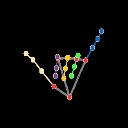
\includegraphics[width=\linewidth]{gambar/pose_prediction_pointer.jpg}
% %     \caption{pointer}
% %     \label{fig:landmarkpointer}
% %   \end{subfigure}
% %   \quad
% %   \begin{subfigure}{0.31\textwidth}
% %     \centering
% %     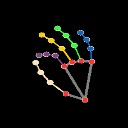
\includegraphics[width=\linewidth]{gambar/pose_prediction_zoom_right.jpg}
% %     \caption{zoom}
% %     \label{fig:landmarkzoom}
% %   \end{subfigure}
% %   \caption{Hasil estimasi pose}
% %   \label{fig:hasilposeprediction}
% % \end{figure}

% \subsection{Hasil Model Klasifikasi}
% \label{subsec:hasilmodelklasifikasi}

% % \begin{longtable}{|c|c|}
% %   \caption{Detail Hyperparameter yang Digunakan}
% %   \label{tb:detailhyperparameteryangdigunakan}\\
% %   \hline
% %   \rowcolor[HTML]{C0C0C0}
% %   \textbf{Weights} & \textbf{CNN} \\
% %   \hline
% %   Class Number            & 6            \\
% %   Epochs                  & 25           \\
% %   Batch-Size              & 16           \\
% %   Image Size              & 128 x 128    \\
% %   Learning rate           & 0.01         \\
% %   Optimizer               & SGD          \\
% %   Jumlah layer konvolusi  & 2            \\
% %   \hline
% % \end{longtable}

% \subsection{Hasil Kontrol PowerPoint}
% \label{subsec:hasilkontrolpowerpoint}

\section{Skenario Pengujian}
\label{sec:skenariopengujian}

Pada tugas akhir ini dilakukan empat skenario pengujian. Pengujian ini diperlukan untuk mengetahui tingkat keberhasilan atau kesalahan agar dapat ditarik kesimpulan yang sesuai. Berikut ini adalah daftar skenario pengujiannya.

\begin{enumerate}[nolistsep]

  \item Pengujian hasil training dan validasi model CNN
  \item Pengujian dengan menggunakan variasi jarak dataset
  \item Pengujian dengan menggunakan variasi Pencahayaan
  \item Pengujian tingkat \emph{Frame Rate}
  \item Pengujian dengan menggunakan tangan dari responden yang berbeda
  \item Pengujian dengan membandingkan model lain (\emph{Resnet50, VGG16,} dan \emph{MobileNet}) 
  \item Pengujian \emph{user experience}

\end{enumerate}

\section{Hasil Pengujian}
\label{sec:hasilpengujian}

Hasil pengujian adalah implementasi dari skenario pengujian yang sudah dijelaskan pada bab 4.2, untuk hasil lengkapnya dapat dilihat pada penjelasan berikut ini.

\subsection{Hasil Pengujian Model}
\label{subsec:hasilpengujianmodel}

\begin{figure}[!htb]
  \centering
  \begin{subfigure}{0.53\textwidth}
    \centering
    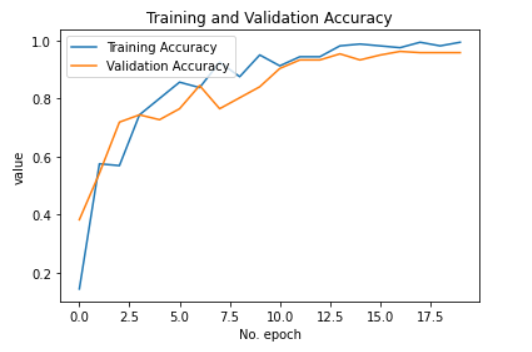
\includegraphics[width=\linewidth]{gambar/training-validation-accuracy.png}
    \caption{Training and Validation Accuracy}
    \label{fig:landmarknextslide} 
  \end{subfigure}
  \begin{subfigure}{0.46\textwidth}
    \centering
    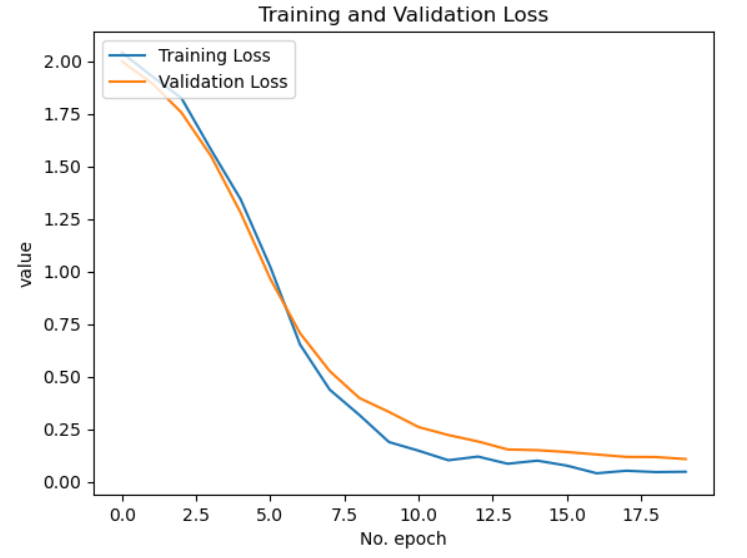
\includegraphics[width=\linewidth]{gambar/training-validation-loss.png}
    \caption{Training and Validation Loss}
    \label{fig:landmarkpreviousslide} 
  \end{subfigure}
  \caption{Hasil Pengujian Model}
  \label{fig:Pengujian Training Validation}
\end{figure}

\hfill \break

Pengujian model bertujuan untuk mengukur akurasi dari model yang dibuat berdasarkan hasil training yang dilakukan menggunakan \emph{library tensorflow}. Akurasi ini dapat diukur dari hasil perhitungan tiap \emph{epoch} yang dilakukan. Grafik pengujian model perbandingan antara akurasi \emph{training} dengan \emph{validation} pada tiap \emph{epoch}, dapat dilihat pada gambar \ref{fig:Pengujian Training Validation}. Training yang dimaksud disini adalah hasil model dari dataset yang dilatih. Sedangkan validation menggunakan dataset yang belum pernah dilihat sebelumnya (berbeda dengan dataset pada training).

Sedangkan untuk perbedaan akurasi dan loss adalah akurasi merupakan banyaknya hasil prediksi yang diklasifikasikan dengan benar. Sedangkan, loss adalah nilai yang menunjukkan perbedaan dari target yang diharapkan. Melalui Grafik \ref{fig:Pengujian Training Validation} didapatkan informasi bahwa nilai akurasi tiap \emph{epoch} menunjukkan adanya peningkatan dari waktu kewaktu. Nilai akurasi \emph{training} akhirnya ada pada 99\%. Sedangkan, untuk akurasi \emph{validation} akhirnya ada pada kisaran 96\%. Performa akurasi model yang hampir sama antara training dan validasi adalah hasil yang baik, karena artinya model dapat memprediksi data yang belum pernah dilihat sebelumnya.

Pada training loss didapatkan nilai dikisaran 0,03. Sedangkan, validation loss dikisaran 0,12. Jarak antara training dan validation dengan nilai loss yang semakin kecil ini menunjukkan prediksi yang error pada model juga kecil.

\subsection{Hasil Pengujian Menggunakan Variasi Jarak}
\label{subsec:Hasil Pengujian Menggunakan Variasi Jarak}

Skenario pengujian menggunakan variasi jarak bertujuan mengukur akurasi dari setiap jarak yang ditentukan. Hal ini dapat menunjukkan seberapa baik kemampuan model dalam mendeteksi klasifikasi pose tangan pada jarak tertentu. Akurasi pengujian model ini diukur dengan membuat data pengujian, dimana data pengujian ini berisi input citra yang diambil diluar dataset. Variasi jarak yang digunakan sendiri dapat dilihat pada Tabel \ref{tb:Gambaran Kondisi Pengujian Jarak} dimana pengujian dilakukan pada jarak 40 cm, 60 cm, 100 cm. Data yang telah didapat dapat dihitung berapa banyak data yang benar sesuai hasil prediksi dan berapa banyak yang tidak sesuai hasil prediksi.

\begin{longtable}{|c|c|c|}
  \caption{Gambaran Kondisi Pengujian Jarak}
  \label{tb:Gambaran Kondisi Pengujian Jarak}\\
  \hline
  \textbf{No.} & \textbf{Jarak (cm)} & \textbf{Gambar Pengujian} \\
  \hline
  \endhead
  1 & \emph{40}  &  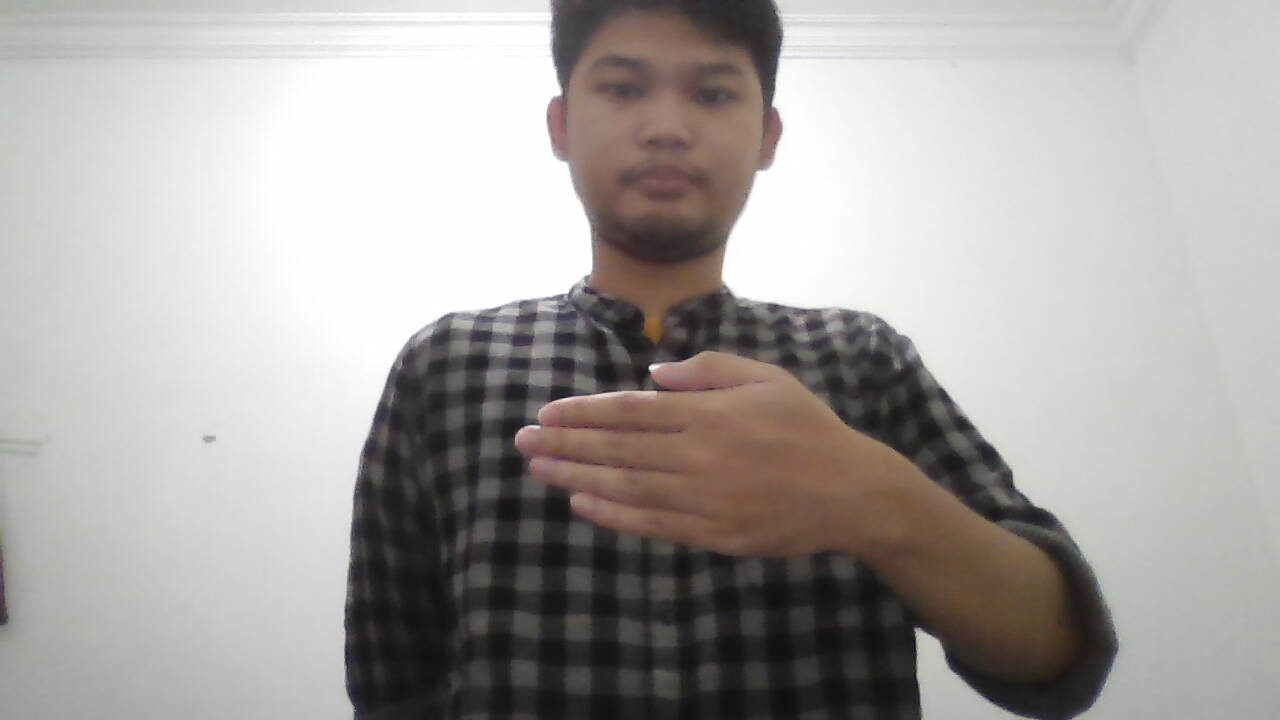
\includegraphics[scale=0.2]{gambar/pengujian-jarak/pengambilan-data/jarak-40cm.jpg} \\
  \hline
  2 & \emph{60}  &  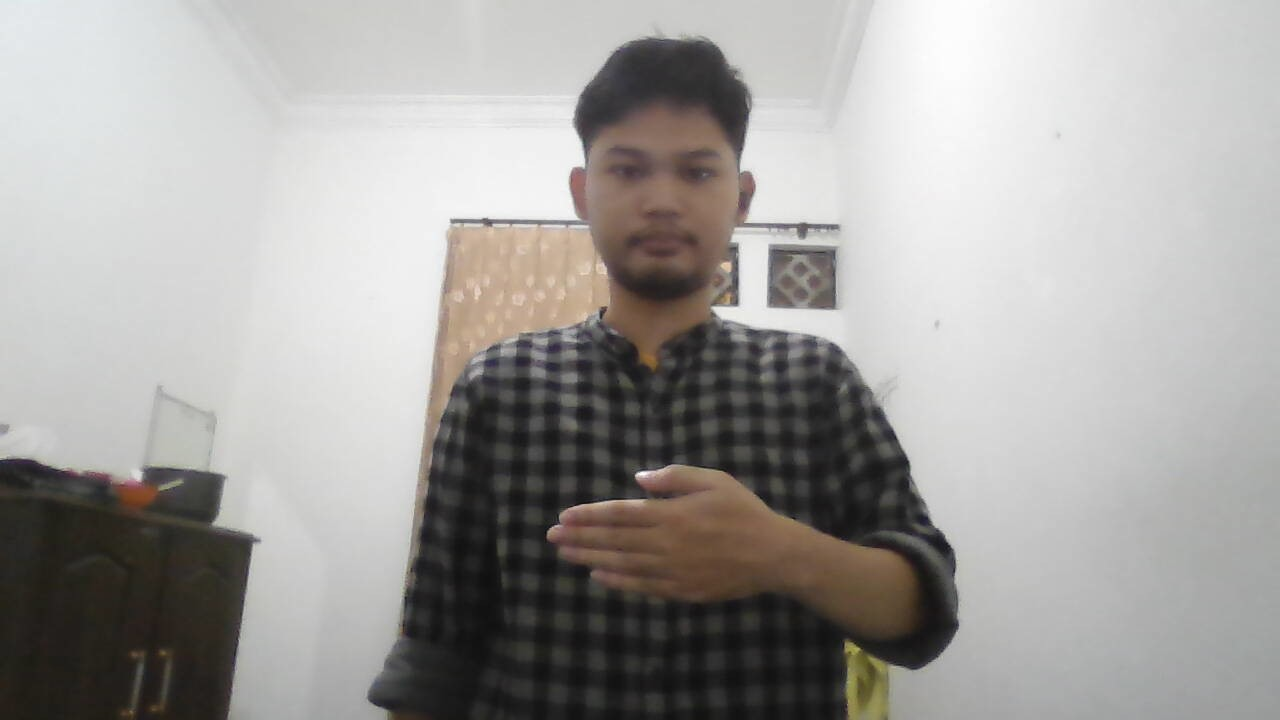
\includegraphics[scale=0.2]{gambar/pengujian-jarak/pengambilan-data/jarak-60cm.jpg} \\
  \hline
  3 & \emph{80}  &  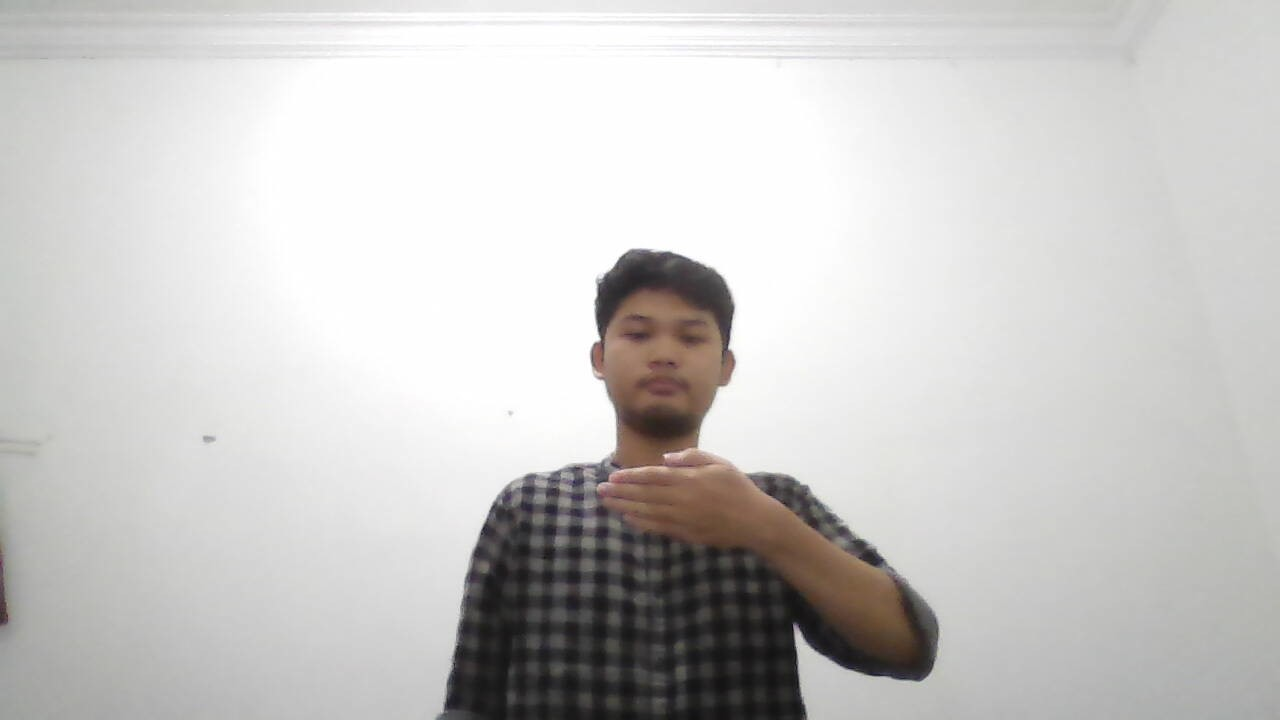
\includegraphics[scale=0.2]{gambar/pengujian-jarak/pengambilan-data/jarak-80cm.jpg} \\
  \hline
  4 & \emph{100}  &  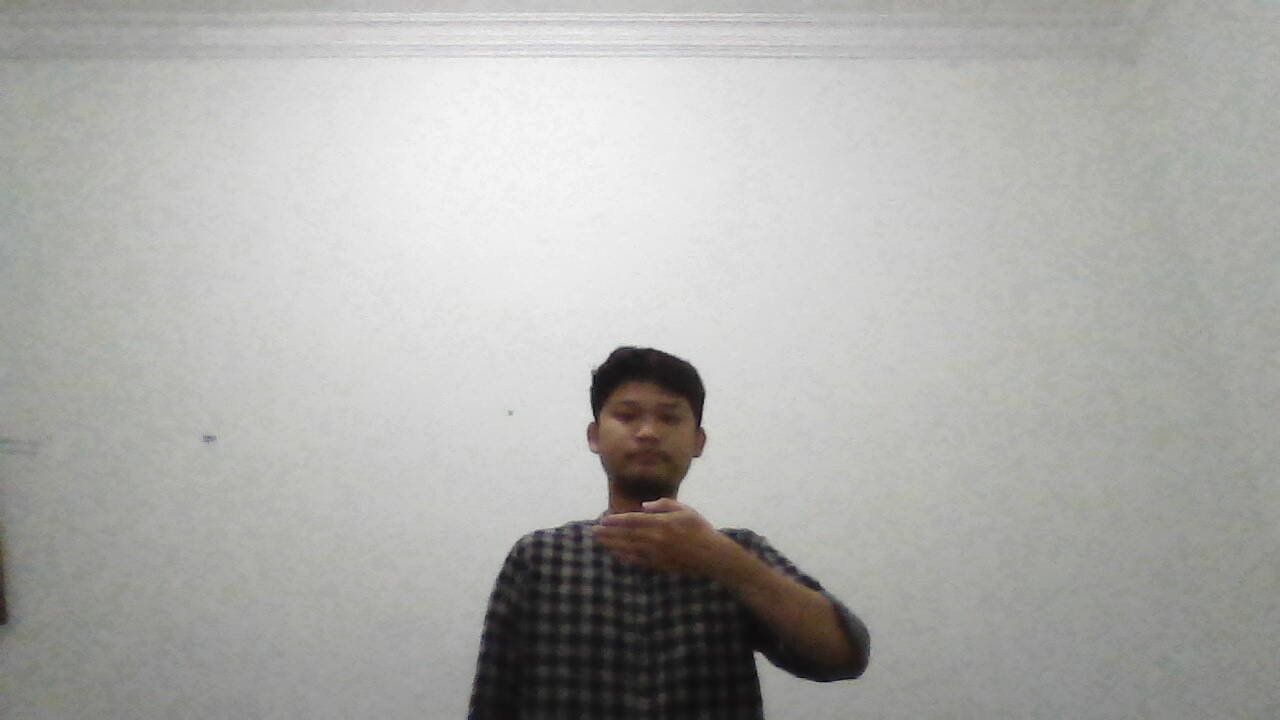
\includegraphics[scale=0.2]{gambar/pengujian-jarak/pengambilan-data/jarak-100cm.jpg} \\
  \hline
\end{longtable}

Pengujian variasi jarak ini diuji dengan menggunakan dua model yang memiliki perbedaan pada datasetnya. Model yang pertama menggunakan kumpulan dataset yang dimana posisi pengambilan datanya bersifat statis disatu jarak tertentu. Jarak yang digunakan dalam model pertama ini adalah sejauh 40 cm. Selain model tersebut, dibuat pula model yang kedua. Model kedua ini menggunakan kumpulan dataset yang posisi pengambilannya bervariasi mulai dari 40 cm hingga 100 cm. Tujuan dilakukannya variasi pengambilan dataset ini untuk diuji apakah model ini dapat mendeteksi lebih baik  dibandingkan dengan model yang hanya menggunakan dataset dengna satu variasi jarak saja. Berikut ini adalah hasil dari pengujian menggunakan variasi jarak.

\subsubsection{Pengujian Menggunakan Dataset Satu Jarak}
\label{subsubsec:Pengujian Menggunakan Dataset Satu Jarak}

Dalam model pertama ini, seperti yang telah disebut dalam bab \ref{subsec:Hasil Pengujian Menggunakan Variasi Jarak} jarak yang digunakan sebagai pengambilan dataset adalah sebesar 40 cm yang berarti ini sama dengan panjang jarak pada variasi yang terdekat. Hasil distribusi prediksi klasifikasi dapat dilihat pada Gambar \ref{fig:Pengujian Tanpa Variasi Jarak Dataset (40 cm)} untuk jarak 40 cm, Gambar \ref{fig:Pengujian Tanpa Variasi Jarak Dataset (60 cm)} untuk jarak 60 cm, Gambar \ref{fig:Pengujian Tanpa Variasi Jarak Dataset (80 cm)} untuk jarak 80 cm, dan Gambar \ref{fig:Pengujian Tanpa Variasi Jarak Dataset (100 cm)}. Hasil distribusinya cukup beragam namun hampir semuanya terdapat kesalahan prediksi yang masuk kedalam kelas \emph{erase}.  

Hasil akurasinya dapat dilihat pada Tabel \ref{tb:Hasil Pengujian Tanpa Variasi Jarak Dataset}. Melalui data tersebut didapatkan hasil bahwa tingkat akurasi yang didapatkan mengalami penurunan setiap jaraknya diperlebar, dimana saat jarak 40 cm didapatkan akurasi sebesar 96.00 \%, saat jarak 60 cm didapatkan akurasi 95.00 \%. Sedangkan saat jarak 80 cm akurasinya sebesar 75.50 \% dan yang terakhir saat jarak 100 cm didapatkan akurasi sebesar 68.00 \%. Berkurangnya akurasi seiring bertambahnya jarak terjadi karena berkurangnya keakuratan titik \emph{landmark} yang dapat dideteksi. Selain itu, bisa diketahui juga bahwa jarak yang paling ideal adalah jarak yang sesuai dengan pengambilan dataset yaitu sebesar 40 cm.

\begin{figure}[!htb]
  \centering
  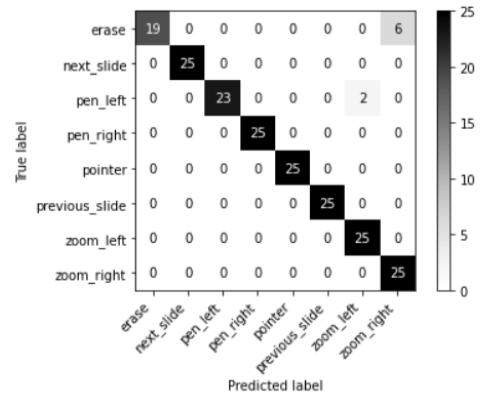
\includegraphics[scale=0.79]{gambar/pengujian-jarak/homogen-dataset/40cm.png}
  \caption{Pengujian Tanpa Variasi Jarak Dataset (40 cm)}
  \label{fig:Pengujian Tanpa Variasi Jarak Dataset (40 cm)}
\end{figure}

\begin{figure}[!htb]
  \centering
  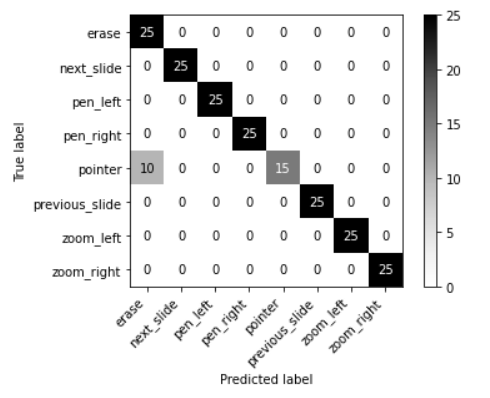
\includegraphics[scale=0.79]{gambar/pengujian-jarak/homogen-dataset/60cm.png}
  \caption{Pengujian Tanpa Variasi Jarak Dataset (60 cm)}
  \label{fig:Pengujian Tanpa Variasi Jarak Dataset (60 cm)}
\end{figure}

\begin{figure}[!htb]
  \centering
  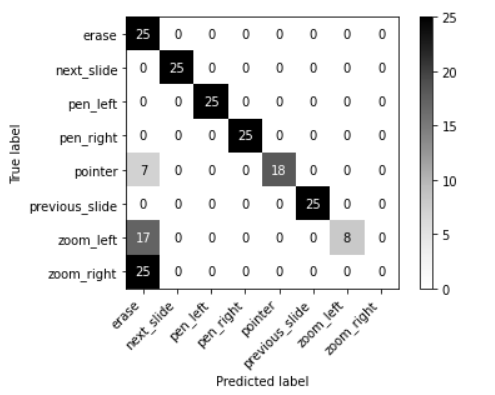
\includegraphics[scale=0.79]{gambar/pengujian-jarak/homogen-dataset/80cm.png}
  \caption{Pengujian Tanpa Variasi Jarak Dataset (80 cm)}
  \label{fig:Pengujian Tanpa Variasi Jarak Dataset (80 cm)}
\end{figure}

\hfill \break
\hfill \break

\begin{figure}[!htb]
  \centering
  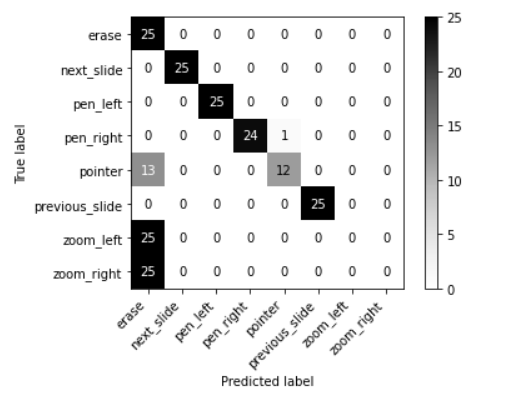
\includegraphics[scale=0.8]{gambar/pengujian-jarak/homogen-dataset/100cm.png}
  \caption{Pengujian Tanpa Variasi Jarak Dataset (100 cm)}
  \label{fig:Pengujian Tanpa Variasi Jarak Dataset (100 cm)}
\end{figure}

\begin{longtable}{|c|c|c|c|c|}
  \caption{Hasil Pengujian Tanpa Variasi Jarak Dataset}
  \label{tb:Hasil Pengujian Tanpa Variasi Jarak Dataset}\\
  \hline
  \rowcolor[HTML]{FFFFFF}
  \textbf{No.} & \textbf{Jarak} & \textbf{Data Terdeteksi Benar} & \textbf{Data Terdeteksi Salah} & \textbf{Akurasi(\%)} \\
  \hline
  1 & 40 cm  & 192 & 8 & 96.00\%  \\
  2 & 60 cm  & 190 & 10 & 95.00\%  \\
  3 & 80 cm  & 151 & 49 & 75.50\%  \\
  4 & 100 cm & 136 & 64 & 68.00\%  \\
  \hline
\end{longtable}

\subsubsection{Pengujian Menggunakan Dataset dengan Jarak Bervariasi}
\label{subsubsec:Pengujian Menggunakan Dataset dengan Jarak Bervariasi}
Dalam pengujian ini, model yang digunakan memiliki dataset yang jaraknya beda-beda. Penulis mengambil dataset tiap kelasnya dengan cara bergerak mulai dari jarak sekitar 40 cm terhadap kamera, dan perlahan-lahan mundur sampai jarak sekitar 100 cm. Hasil distribusi tiap kelasnya dapat dilihat pada Gambar \ref{fig:Pengujian Dataset dengan Variasi Jarak (40 cm)}, \ref{fig:Pengujian Dataset dengan Variasi Jarak (60 cm)}, \ref{fig:Pengujian Dataset dengan Variasi Jarak (60 cm)}, dan \ref{fig:Pengujian Dataset dengan Variasi Jarak (100 cm)}. Persebaran prediksi klasifikasinya lebih stabil dan umumnya berada pada kelas yang benar apabila dibandingkan dengan dataset tanpa variasi jarak. 

Dalam pengujian dengan jarak dataset yang bervariasi ini didapatkan ringkasan hasil data seperti pada Tabel \ref{tb:Hasil Pengujian Dataset dengan Variasi Jarak}. Berdasarkan data tersebut didapatkan hasil bahwa tingkat akurasi memang mengalami penurunan setiap jaraknya diperlebar. Namun, akurasi yang dihasilkan masih tetap lebih tinggi dibanding model sebelumnya. 

Saat jarak 40 cm didapatkan akurasi sebesar 99.00\%, saat jarak 60 cm didapatkan akurasi 97.50\%, Kemudian saat jarak 80 cm akurasinya sebesar 97.00\%, dan saat jarak 100 cm didapatkan akurasi sebesar 94.50\%. Dari data ini dapat diketahui bahwa variasi jarak pada dataset sangat mempengaruhi akurasi apabila pengambilan data citra dilakukan dengan jarak yang bervariasi juga.

\begin{figure}[!htb]
  \centering
  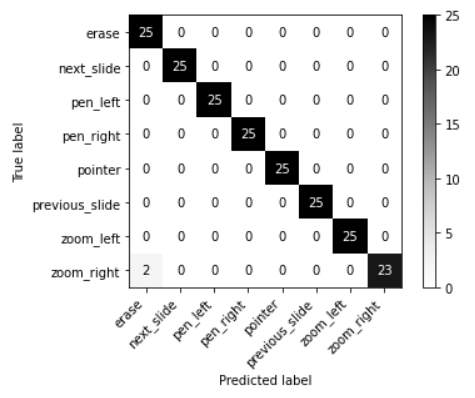
\includegraphics[scale=0.78]{gambar/pengujian-jarak/heterogen-dataset/40cm.png}
  \caption{Pengujian Dataset dengan Variasi Jarak (40 cm)}
  \label{fig:Pengujian Dataset dengan Variasi Jarak (40 cm)}
\end{figure}

\begin{figure}[!htb]
  \centering
  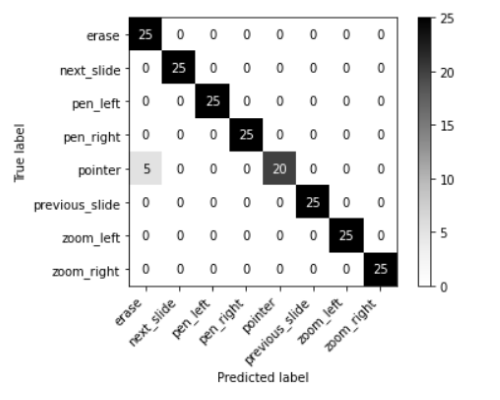
\includegraphics[scale=0.78]{gambar/pengujian-jarak/heterogen-dataset/60cm.png}
  \caption{Pengujian Dataset dengan Variasi Jarak (60 cm)}
  \label{fig:Pengujian Dataset dengan Variasi Jarak (60 cm)}
\end{figure}

\begin{figure}[!htb]
  \centering
  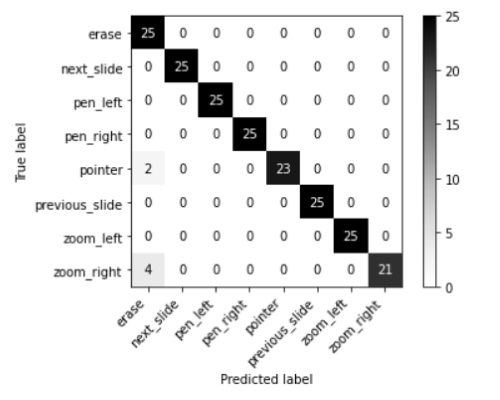
\includegraphics[scale=0.78]{gambar/pengujian-jarak/heterogen-dataset/80cm.png}
  \caption{Pengujian Dataset dengan Variasi Jarak (80 cm)}
  \label{fig:Pengujian Dataset dengan Variasi Jarak (80 cm)}
\end{figure}

\hfill \break
\hfill \break
\hfill \break
\hfill \break

\begin{figure}[!htb]
  \centering
  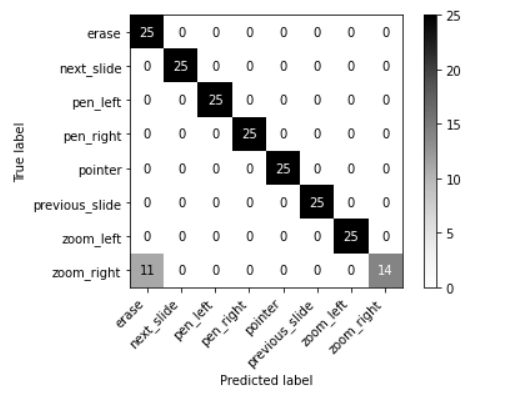
\includegraphics[scale=0.8]{gambar/pengujian-jarak/heterogen-dataset/100cm.png}
  \caption{Pengujian Dataset dengan Variasi Jarak (100 cm)}
  \label{fig:Pengujian Dataset dengan Variasi Jarak (100 cm)}
\end{figure}

\begin{longtable}{|c|c|c|c|c|}
  \caption{Hasil Pengujian Dataset dengan Variasi Jarak}
  \label{tb:Hasil Pengujian Dataset dengan Variasi Jarak}\\
  \hline
  \rowcolor[HTML]{FFFFFF}
  \textbf{No.} & \textbf{Jarak} & \textbf{Data Terdeteksi Benar} & \textbf{Data Terdeteksi Salah} & \textbf{Akurasi(\%)} \\
  \hline
  1 & 40 cm  & 198 & 2 & 99.00\%  \\
  2 & 60 cm  & 195 & 5 & 97.50\%  \\
  3 & 80 cm  & 194 & 6 & 97.00\%  \\
  4 & 100 cm & 189 & 11 & 94.50\%  \\
  \hline
\end{longtable}

\subsection{Hasil Pengujian Menggunakan Variasi Pencahayaan}
\label{subsec:Hasil Pengujian Menggunakan Variasi Pencahayaan}

\begin{figure}[!htb]
  \centering
  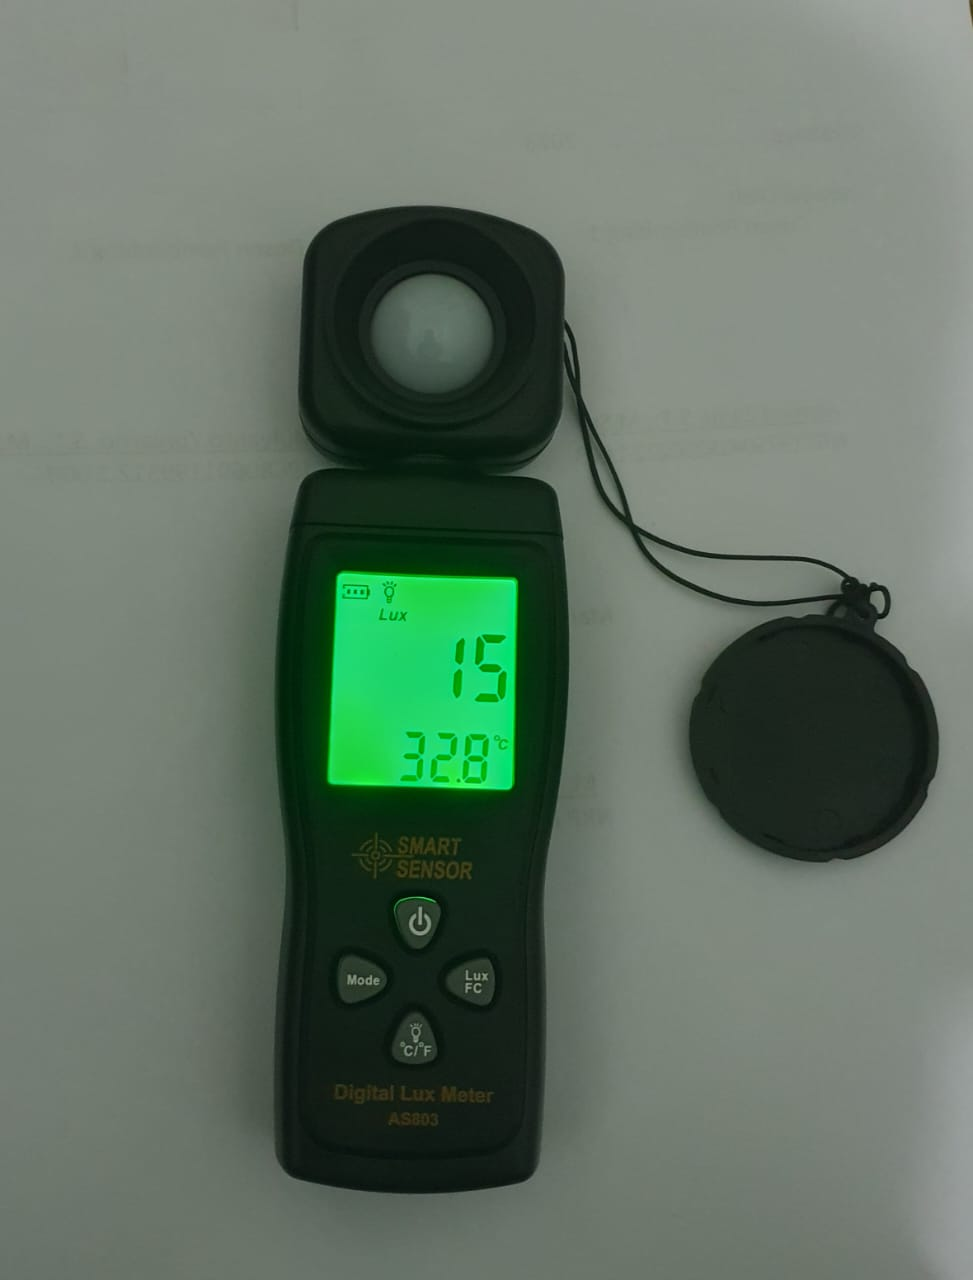
\includegraphics[scale=0.15]{gambar/lux-meter.jpeg}
  \caption{\emph{Digital Lux Meter}}
  \label{fig:Digital Lux Meter}
\end{figure}

Pengujian menggunakan variasi Pencahayaan yang berbeda-beda ini dilakukan dengan tujuan untuk menguji performa tingkat keterbacaan pose tangan dalam berbagai kondisi cahaya di tempat pengambilan citra. Dalam mengukur pencahayaan ini sendiri digunakan alat ukur bernama \emph{Digital Lux Meter}, yang dapat dilihat pada Gambar \ref{fig:Digital Lux Meter}. \emph{Lux Meter} merupakan perangkat yang mengukur banyaknya cahaya masuk menggunakan satuan lux dalam perhitungannya. Satuan lux sendiri adalah besarnya arus cahaya yang datang persatuan luas permukaan. Sehingga, alat ini dapat menjadi acuan tiap kondisi pencahayaan dalam skenario pengujian kali ini.

Variasi pencahayaannya dibagi menjadi tiga kondisi. Kondisi pertama adalah didalam ruangan yang mendapat cahaya lampu dengan cerah. Jika diukur dengan \emph{lux meter} nilainya pada kisaran 40 lx. Kondisi kedua adalah pencahayaan yang redup, dimana pengujian diambil tetap dalam ruangan namun kondisi lampu mati dan hanya memanfaatkan cahaya matahari dari celah-celah jendela dan pintu ruangan. Apabila diukur dengan \emph{lux meter} didapatkan angka sebesar 15 lx. Kondisi terakhir adalah kondisi pencahayaan gelap, dimana pengujian dilakukan dalam ruangan tanpa cahaya lampu dan matahari. Sumber cahaya yang ada hanya dari layar laptop. Dalam kondisi ketiga ini didapatkan angka pada \emph{lux meter} sebesar 5 lx. Gambaran kondisi pengambilan data pengujian untuk kondisi terang dapat dilihat pada gambar \ref{fig:kondisi_40lux}, kondisi redup pada gambar \ref{fig:kondisi_15lux}, dan kondisi gelap pada gambar \ref{fig:kondisi_5lux}.

\begin{figure}[!htb]
  \centering
  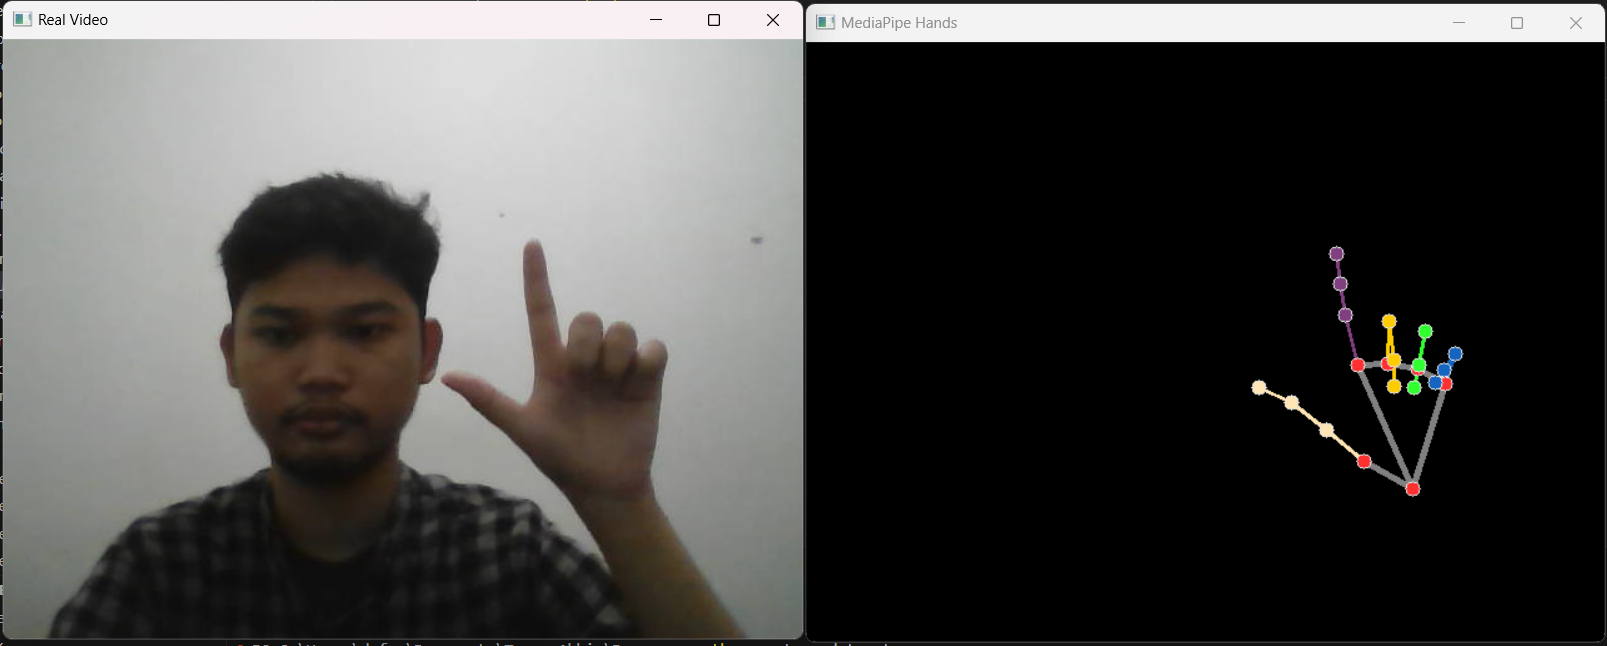
\includegraphics[scale=0.4]{gambar/pengujian-cahaya/kondisi_40lux.png}
  \caption{Kondisi Terang(40 lx)}
  \label{fig:kondisi_40lux} 
\end{figure}

\begin{figure}[!htb]
  \centering
  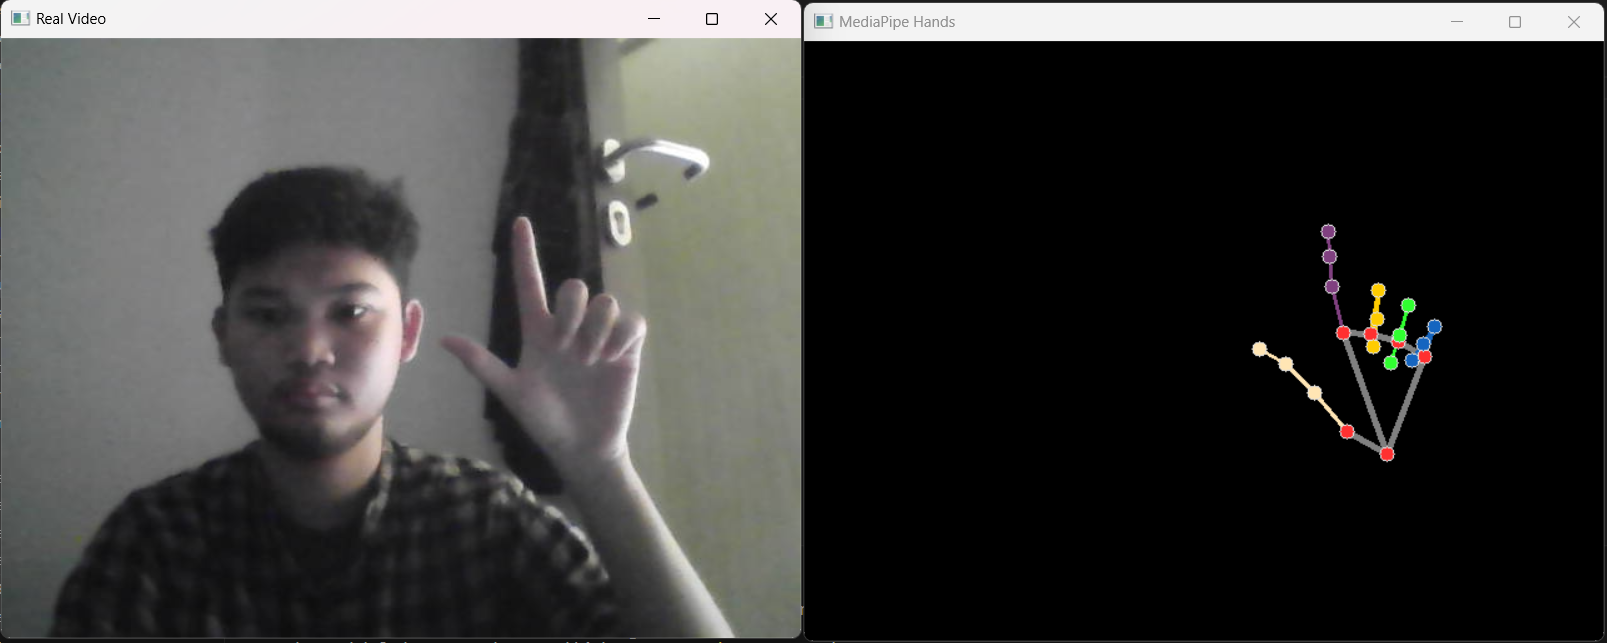
\includegraphics[scale=0.4]{gambar/pengujian-cahaya/kondisi_15lux.png}
  \caption{Kondisi Terang(15 lx)}
  \label{fig:kondisi_15lux} 
\end{figure}

\hfill \break

\begin{figure}[!htb]
  \centering
  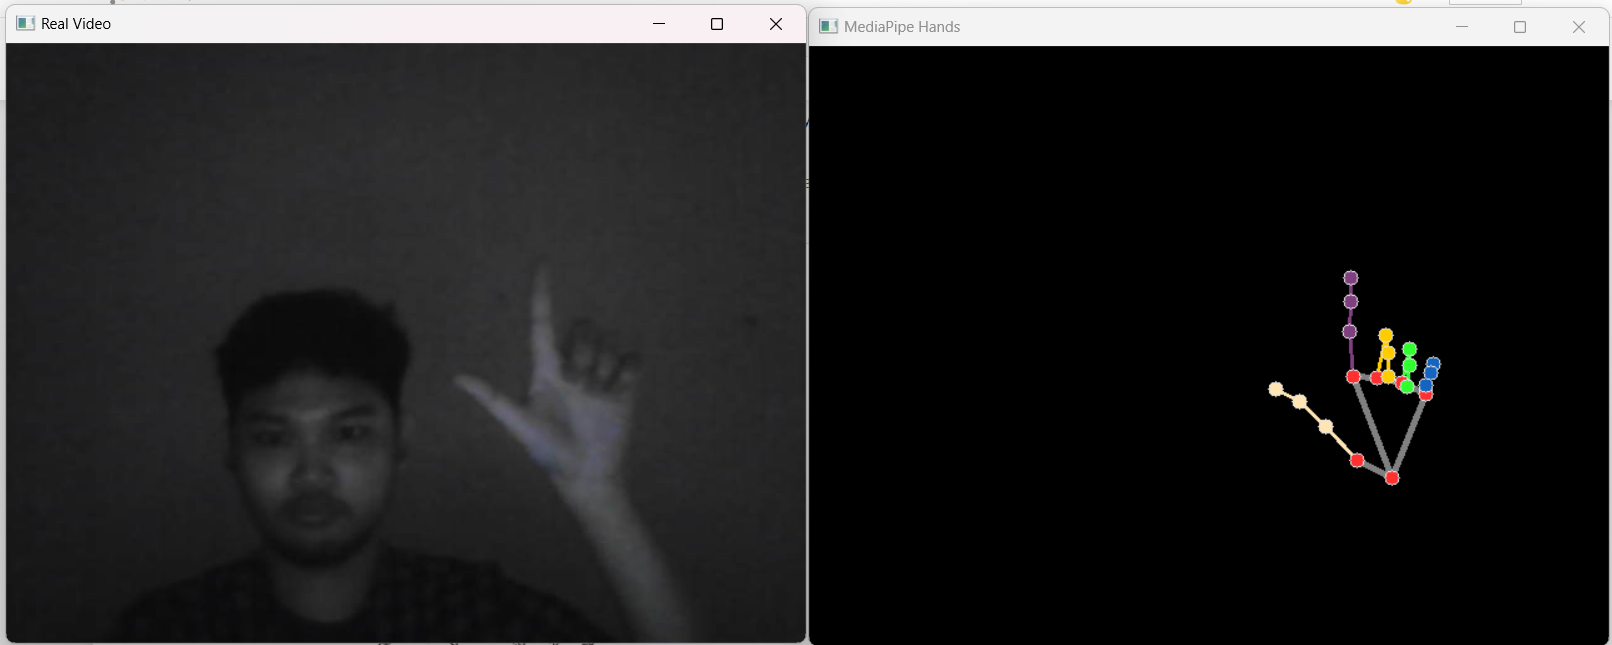
\includegraphics[scale=0.4]{gambar/pengujian-cahaya/kondisi_5lux.png}
  \caption{Kondisi Terang(5 lx)}
  \label{fig:kondisi_5lux} 
\end{figure}

Persebaran hasil klasifikasi yang benar dan salah untuk pencahayaan kondisi gelap ada pada Gambar \ref{fig:Pengujian Dataset dengan Variasi Pencahayaan 5lux}. Hasil klasifikasi dimana citra yang sebenarnya termasuk klasifikasi \emph{'pointer'} tapi salah terdeteksi kedalam \emph{'erase'}. Hal ini bisa terjadi karena dikondisi gelap terkadang ada bagian yang terjadi kesalahan prediksi. Pada citra \emph{'pointer'} misalnya, bagian jari kelingking dan jempol yang tidak terdeteksi. Sehingga, pose pointer jadi terlihat seperti pose \emph{'erase'}. Hal inilah yang menyebabkan terdapat 14 citra \emph{'pointer'} yang salah terdeteksi kedalam kelas \emph{'erase'}. 

Berdasarkan pengujian yang dilakukan, didapatkan data seperti yang tertera dalam tabel \ref{tb:Hasil Pengujian dengan Variasi Pencahayaan}. Dalam data tersebut menunjukkan bahwa dalam kondisi cahaya terang, tingkat akurasi yang dicapai sebesar 99.00\%. Sedangkan untuk kondisi cahaya redup akurasinya yang didapatkan sebesar 96.00\%. Terakhir, dalam kondisi pencahayaan gelap akurasinya sebesar 89.00\%. Melalui data tersebut memang terjadi penurunan akurasi saat setiap kondisi pencahayaan semakin menurun. 

Namun, penurunan akurasi yang terjadi tidak terlalu signifikan, bahkan sampai dalam kondisi pencahayaan sangat gelap sekalipun. Hal ini lebih banyak dipengaruhi faktor kemampuan dalam \emph{library mediapipe}. Selama \emph{mediapipe} masih dapat mendeteksi \emph{landmark} tangan dengan tepat, maka model klasifikasi pun juga tetap mampu memprediksi pose dengan tepat juga. Karena, yang dibaca oleh model adalah \emph{landmark} tangan yang sudah diproses \emph{mediapipe}, bukan gambar pose tangan langsung dari kamera. 

\begin{figure}[!htb]
  \centering
  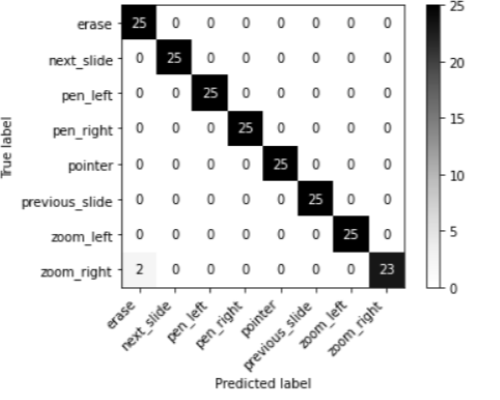
\includegraphics[scale=0.7]{gambar/pengujian-cahaya/40lux.png}
  \caption{Pengujian Dataset dengan Variasi Pencahayaan (40 lx)}
  \label{fig:Pengujian Dataset dengan Variasi Pencahayaan 40lux} 
\end{figure}

\begin{figure}[!htb]
  \centering
  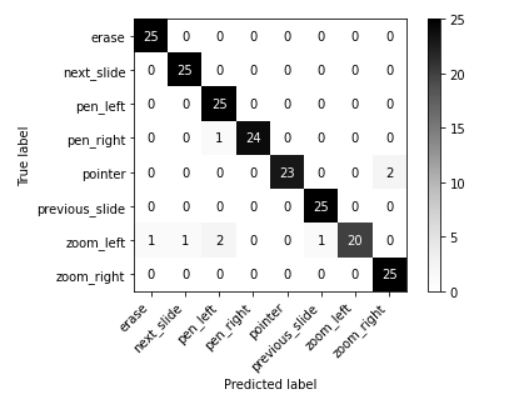
\includegraphics[scale=0.75]{gambar/pengujian-cahaya/15lux.png}
  \caption{Pengujian Dataset dengan Variasi Pencahayaan (15 lx)}
  \label{fig:Pengujian Dataset dengan Variasi Pencahayaan 15lux} 
\end{figure}

\begin{figure}[!htb]
  \centering
  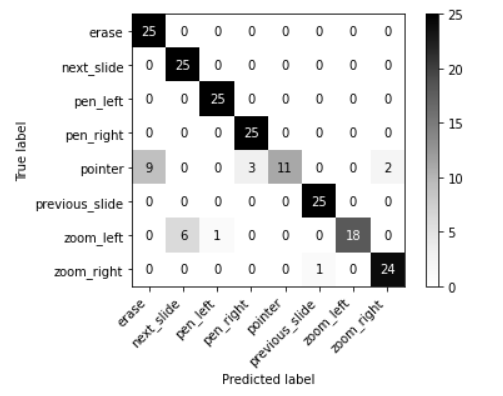
\includegraphics[scale=0.75]{gambar/pengujian-cahaya/5lux.png}
  \caption{Pengujian Dataset dengan Variasi Pencahayaan (5 lx)}
  \label{fig:Pengujian Dataset dengan Variasi Pencahayaan 5lux} 
\end{figure}

\begin{longtable}{|c|c|c|c|c|}
  \caption{Hasil Pengujian dengan Variasi Pencahayaan}
  \label{tb:Hasil Pengujian dengan Variasi Pencahayaan}\\
  \hline
  \rowcolor[HTML]{FFFFFF}
  \textbf{No.} & \textbf{Cahaya} & \textbf{Data Terdeteksi Benar} & \textbf{Data Terdeteksi Salah} & \textbf{Akurasi(\%)} \\
  \hline
  1 & Terang (40 lx)  & 198 & 2 & 99.00\%  \\
  2 & Redup (15 lx)   & 192 & 8 & 96.00\%  \\
  3 & Gelap (5 lx)    & 178 & 22 & 89.00\%  \\
  \hline
\end{longtable}

\subsection{Hasil Pengujian \emph{Frame Rate}}
\label{subsec:Hasil Pengujian Frame Rate}

\emph{Frame Rate} pada umumnya dinyatakan dalam satuan per detik atau disebut sebagai \emph{Frame Per Second (FPS)}. FPS ini merupakan pengukuran seberapa banyak jumlah frame yang ada dalam satu detik. Pengujian \emph{Frame Rate} dianggap penting karena menjadi salah satu penilaian performa dari model yang dibuat. Selain itu, \emph{Frame Rate} juga sangat mempengaruhi penilaian \emph{user experience}. Apabila semakin kecil nilainya maka gerakan semakin terlihat patah-patah, dan respon yang diberikan semakin lambat. Sebaliknya, semakin besar nilainya maka  gerakan yang dihasilkan lebih lancar dan responnya semakin cepat.

\newpage

\begin{figure}[!htb]
  \centering
  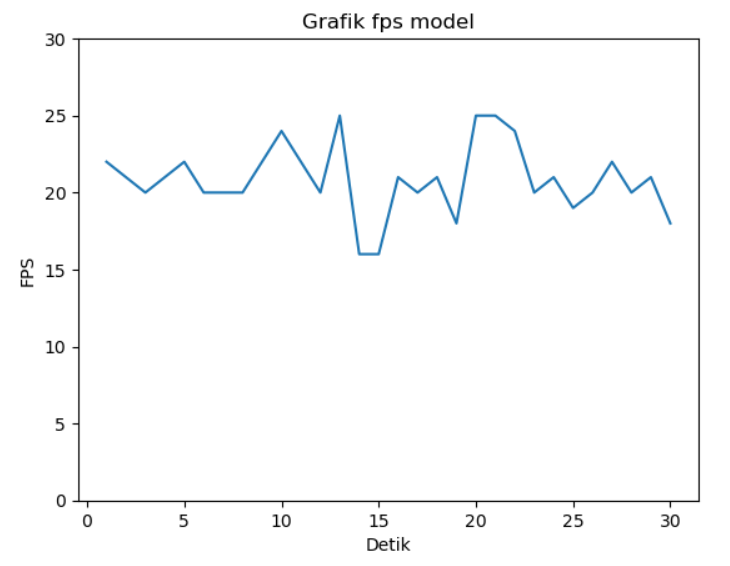
\includegraphics[scale=0.7]{gambar/pengujian-fps/grafik-pengujian-fps.png}
  \caption{Grafik Pengujian \emph{Frame Rate}}
  \label{fig:Grafik Pengujian Frame Rate}
\end{figure}

Pada pengujian kali ini, perhitungan \emph{frame rate} diuji dengan mengambil data nilai FPS setiap detiknya selama 30 detik pada kondisi ideal yaitu cahaya terang dan jarak sekitar 40 cm - 60 cm. Hasil pengujian \emph{frame rate} dapat dilihat pada gambar \ref{fig:Grafik Pengujian Frame Rate}. Berdasarkan grafik pada Gambar \ref{fig:Grafik Pengujian Frame Rate}, didapatkan nilai rata-rata FPS yang didapatkan sebesar 20.86 FPS, dengan rincian nilai tertingginya bisa mencapai 25 FPS, dan titik terendahnya mendekati 15 FPS. Berdasarkan data ini dapat dinyatakan bahwa performa model memungkinkan untuk masih dapat mendeteksi pose tangan dengan baik. 

\subsection{Hasil Pengujian dari Responden yang Berbeda}
\label{subsec:Hasil Pengujian dari Responden yang Berbeda}
Saat pengambilan dataset untuk proses \emph{training} model, data yang digunakan hanya menggunakan pose tangan penulis saja. Sehingga, perlu dilakukan pengujian apabila pose tangan yang dideteksi merupakan tangan selain penulis yang mungkin secara ukuran berbeda. Hal ini bertujuan untuk mengetahui tingkat akurasi model apabila tangan yang dideteksi memiliki ukuran atau bentuk yang tidak sama dengan tangan penulis yang dijadikan dataset.

Dalam pengujian ini, kondisi pengambilan data responden dilakukan dikondisi ideal. Kondisi ideal yang dimaksud disini adalah kondisi dengan tingkat akurasi paling tinggi yang sudah diuji dalam skenario pengujian pada subbab \ref{subsec:Hasil Pengujian Menggunakan Variasi Jarak} dan \ref{subsec:Hasil Pengujian Menggunakan Variasi Pencahayaan}. Berdasarkan data tersebut, didapatkan bahwa kondisi paling ideal adalah saat jarak tangan dengan kamera diangka 40 cm. Sedangkan, untuk kondisi cahayanya dilakukan didalam ruangan yang terang (sekitar 40 lx). Berikut ini adalah hasil pengujiannya.

\subsubsection{Pengujian Menggunakan Data Citra dari Responden 1}
\label{subsec:Pengujian Menggunakan Data Citra dari Responden 1}

Pada saat pengambilan data citra, responden 1 diposisikan untuk berada pada kondisi dengan tingkat akurasi paling ideal, dan diambil data citra sebanyak 25 frame pada tiap kelasnya, yang berarti total data citra yang diambil sebanyak 200 data. Berdasarkan gambar \ref{fig:Pengujian Menggunakan Data Citra dari Responden 1} didapatkan tingkat akurasi yang dihasilkan sebesar 88.00\%. Hal ini berarti menunjukkan adanya penurunan akurasi dari model dengan input citra dari penulis. Namun, penurunan yang terjadi tidak terlalu jauh, sehingga masih input citra masih dapat terdeteksi dengan akurasi cukup baik. 

\begin{figure}[!htb]
  \centering
  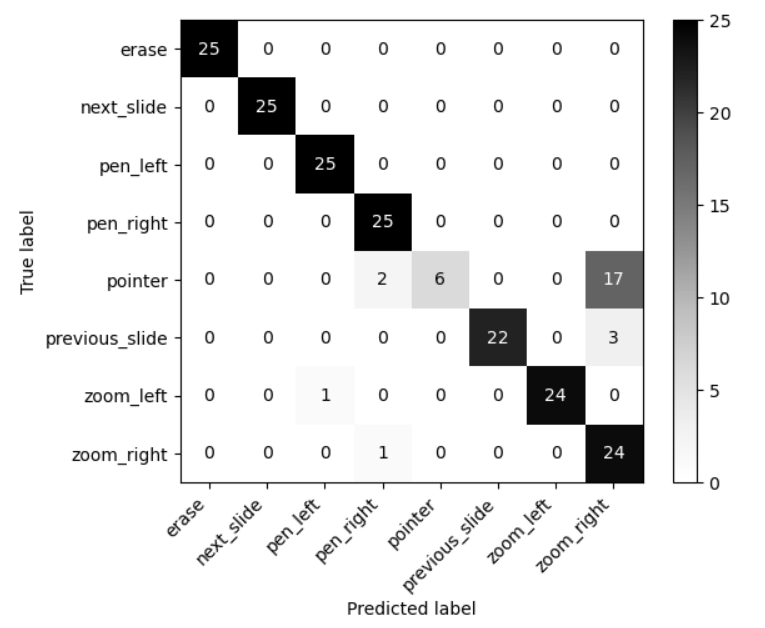
\includegraphics[scale=0.5]{gambar/pengujian-ukuran-tangan/tangan-alfan.png}
  \caption{Pengujian Menggunakan Data Citra dari Responden 1}
  \label{fig:Pengujian Menggunakan Data Citra dari Responden 1}
\end{figure}

\subsubsection{Pengujian Menggunakan Data Citra dari Responden 2}
\label{subsec:Pengujian Menggunakan Data Citra dari Responden 2}

Kondisi pengambilan data citra untuk responden 2, sama dengan responden satu yaitu diposisikan untuk berada pada kondisi dengan tingkat akurasi paling ideal. Jumlah data citra yang diambil juga sebanyak 25 frame pada tiap kelasnya, sehingga total data citranya sebanyak 200 data. Hasilnya dapat dilihat pada gambar \ref{fig:Pengujian Menggunakan Data Citra dari Responden 2}. Didapatkan tingkat akurasi yang dihasilkan sebesar 99.50\%. Hal ini berarti menunjukkan adanya penurunan akurasi dari model dengan input citra dari penulis. Namun, penurunan yang terjadi tidak terlalu jauh, dan bahkan lebih baik dibandingkan dengan responden 1. 

\begin{figure}[ht]
  \centering
  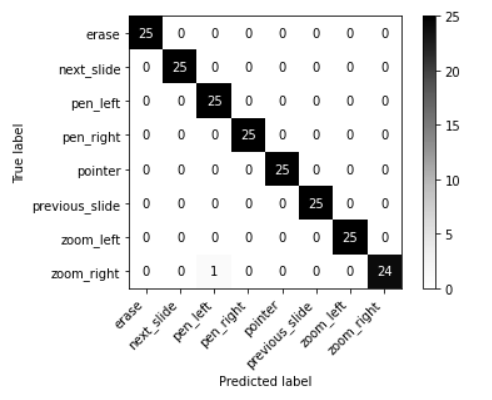
\includegraphics[scale=0.85]{gambar/pengujian-ukuran-tangan/tangan-ari.png}
  \caption{Pengujian Menggunakan Data Citra dari Responden 2}
  \label{fig:Pengujian Menggunakan Data Citra dari Responden 2}
\end{figure}

\subsubsection{Pengujian Menggunakan Data Citra dari Responden 3}
\label{subsec:Pengujian Menggunakan Data Citra dari Responden 3}

Pengambilan data pengujian dilakukan sebanyak 25 citra tiap kelasnya yang diambil pada kondisi ideal. Hasilnya dapat dilihat pada gambar \ref{fig:Pengujian Menggunakan Data Citra dari Responden 3}. Didapatkan tingkat akurasi yang dihasilkan sebesar 86,50\%. Sama dengan responden 1 terdapat adanya penurunan akurasi dari model dengan input citra dari penulis, walaupun masih lebih besar dari 80\%. 

\begin{figure}[ht]
  \centering
  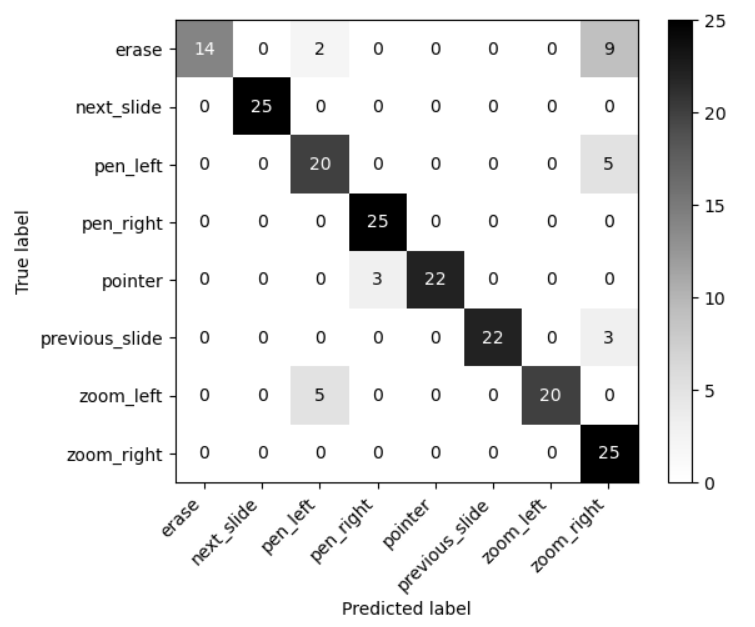
\includegraphics[scale=0.5]{gambar/pengujian-ukuran-tangan/tangan-meril.png}
  \caption{Pengujian Menggunakan Data Citra dari Responden 3}
  \label{fig:Pengujian Menggunakan Data Citra dari Responden 3}
\end{figure}

\subsubsection{Pengujian Menggunakan Data Citra dari Responden 4}
\label{subsec:Pengujian Menggunakan Data Citra dari Responden 4}

Proses pengambilan data citra sama dengan responden sebelumnya, yang dilakukan pada kondisi dengan tingkat akurasi paling ideal. Jumlah data yang digunakan juga sama persis. Hasilnya dapat dilihat pada gambar \ref{fig:Pengujian Menggunakan Data Citra dari Responden 4}. Didapatkan tingkat akurasi yang dihasilkan sebesar 89,50\%. Hal ini berarti menunjukkan adanya penurunan akurasi dari model dengan input citra dari penulis, walaupun akurasinya masih mendekati 90\%.

\begin{figure}[ht]
  \centering
  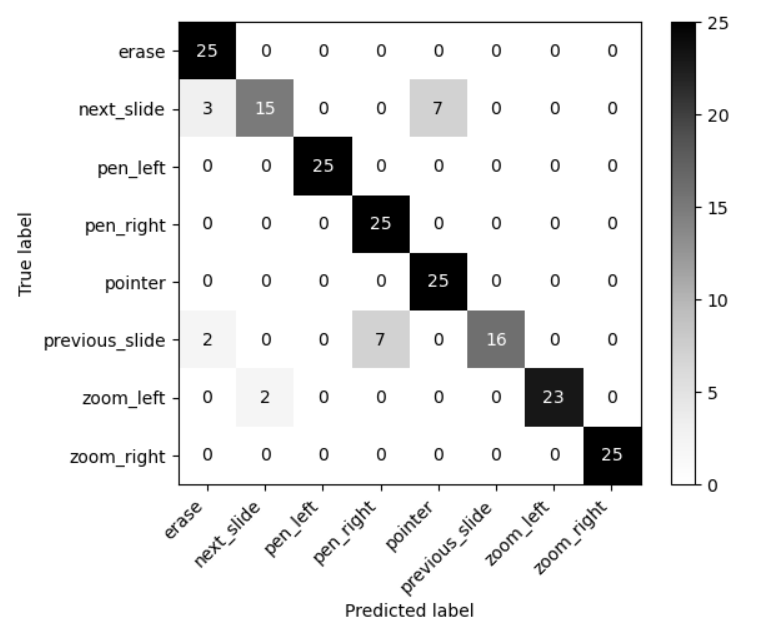
\includegraphics[scale=0.5]{gambar/pengujian-ukuran-tangan/tangan-bakar.png}
  \caption{Pengujian Menggunakan Data Citra dari Responden 4}
  \label{fig:Pengujian Menggunakan Data Citra dari Responden 4}
\end{figure}

Berdasarakan data dari keempat responden yang diambil, dapat diambil ringkasan seperti yang terlihat pada tabel \ref{tb:Hasil Pengujian dengan Variasi Ukuran Tangan}. Memang terjadi adanya penurunan akurasi apabila dibandingkan antara tangan penulis dengan menggunakan tangan responden. Namun, penurunan yang terjadi tidak signifikan, dimana saat menggunakan tangan penulis akurasi yang didapatkan sebesar 98.00\%, sedangkan saat menggunakan tangan responden lain didapatkan rata-rata akurasi sebesar 90.00\%. 

\begin{longtable}{|c|c|c|c|c|}
  \caption{Hasil Pengujian dengan Variasi Ukuran Tangan}
  \label{tb:Hasil Pengujian dengan Variasi Ukuran Tangan}\\
  \hline
  \rowcolor[HTML]{FFFFFF}
  \textbf{No.} & \textbf{Responden} & \textbf{Data Terdeteksi Benar} & \textbf{Data Terdeteksi Salah} & \textbf{Akurasi(\%)} \\
  \hline
  1 & Responden 1  & 179 & 21 & 88,00  \\
  2 & Responden 2  & 168 & 32 & 99,50  \\
  3 & Responden 3  & 190 & 10 & 86,50  \\
  4 & Responden 4  & 190 & 10 & 89,50  \\
  \hline
\end{longtable}

\subsection{Pengujian Menggunakan Model CNN yang Berbeda}
Pengujian ini bertujuan untuk menguji performa apabila menggunakan model yang lain. Terdapat tiga model yang digunakan yaitu Resnet50, VGG16, dan MobileNet. Pengujian ini dilakukan dengan menguji semua variasi yang sama dengan model yang penulis buat sendiri. Berikut adalah hasil pengujian tiap modelnya.

\subsection{Pengujian Menggunakan Model Resnet50}
\label{subsec:Pengujian Menggunakan Model Resnet50}

Pada pengujian pertama, model yang digunakan untuk diuji performanya adalah ResNet50. Model ResNet diusulkan dengan penggunaan metode bernama \emph{Deep Residual Learning for Image Recognition} oleh Kaiming He, Xiangyu Zhang, Shaoqing Ren dan Jian Sun. Model ini memiliki jumlah layer yang jauh lebih banyak dibandingkan model yang dibuat penulis, yaitu berjumlah 50 layer \parencite{Kaiming2015}. Hasil pengujiannya dapat dilihat pada Tabel \ref{tb:Hasil Pengujian Menggunakan model ResNet50}.

\newcolumntype{M}[1]{>{\centering\arraybackslash}m{#1}}

\begin{longtable}[!htb]{|M{25mm}|M{30mm}|M{30mm}|M{30mm}|c|}
  \caption{Hasil Pengujian Menggunakan model ResNet50}
  \label{tb:Hasil Pengujian Menggunakan model ResNet50}\\
  \hline
  \endhead
    Variasi Pengujian & Total Data untuk testing & Data Terprediksi Benar & Data Terprediksi Salah & Akurasi(\%) \\ \hline
    Pengujian Jarak 40 cm & 200 & 195 & 5 & 97.5 \\ \hline
    Pengujian Jarak 60 cm & 200 & 190 & 10 & 95 \\ \hline
    Pengujian Jarak 80 cm & 200 & 195 & 5 & 97.5 \\ \hline
    Pengujian Jarak 100 cm & 200 & 190 & 10 & 95 \\ \hline
    Pengujian Cahaya Terang & 200 & 189 & 11 & 97.5 \\ \hline
    Pengujian \newline Cahaya Redup & 200 & 190 & 10 & 95 \\ \hline
    Pengujian Cahaya Gelap & 200 & 195 & 5 & 94.5 \\ \hline
    Pengujian Menggunakan Tangan Responden 1 & 200 & 183 & 17 & 91.5 \\ \hline
    Pengujian Menggunakan Tangan Responden 2 & 200 & 174 & 26 & 87 \\ \hline
    Pengujian Menggunakan Tangan Responden 3 & 200 & 187 & 13 & 93.5 \\ \hline
    Pengujian Menggunakan Tangan Responden 4 & 200 & 186 & 14 & 93 \\ \hline
\end{longtable}

Berdasarkan Tabel \ref{tb:Hasil Pengujian Menggunakan model ResNet50}, dalam pengujian jarak mendapatkan hasil akurasi rata-rata sebesar 96,25\%, dimana akurasi tertingginya ada pada angka 97,5\% dan terendahnya 95\%. Hasil ini tidak jauh dibandingkan dengan model yang penulis buat yang tercantum dalam Tabel \ref{tb:Hasil Pengujian Dataset dengan Variasi Jarak}, dimana rata-rata yang didapatkan sebesar 97.5\%.

Sedangkan, untuk pengujian cahaya akurasi sama dengan model yang penulis buat yang dimana akurasinya mengalami penurunan seiring dengan kurangnya cahaya yang masuk. Namun untuk kondisi yang sangat gelap, akurasinya terhitung lebih baik dibandingkan model yang dibuat penulis dimana akurasinya sebesar 94.5\% dibandingkan dengan 89.00\%.

Jenis pengujian yang terakhir adalah menggunakan tangan responden yang berbeda-beda. Akurasi yang dihasilkan lebih besar dari model yang penulis buat. Rata-rata yang didapatkan model ini adalah sebesar 91,25\% dibandingkan dengan 90.00\%.

\begin{figure}[!htb]
  \centering
  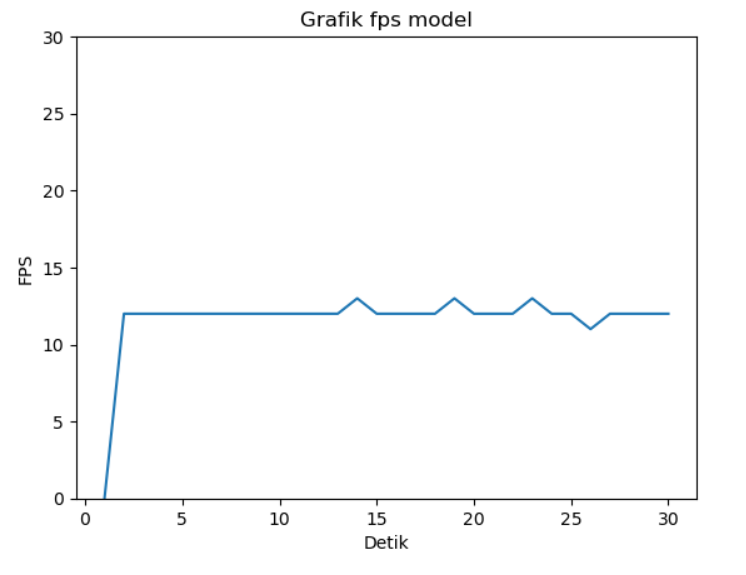
\includegraphics[scale=0.74]{gambar/pengujian-fps/grafik-pengujian-fps-resnet.png}
  \caption{Grafik Pengujian \emph{Frame Rate} Model Resnet50}
  \label{fig:Grafik Pengujian Frame Rate Model Resnet50}
\end{figure}

Selain pengujian yang disebutkan pada Tabel \ref{tb:Hasil Pengujian Menggunakan model ResNet50}, terdapat pengujian \emph{frame rate} untuk mengukur performa model dalam memprediksi citra. Hasilnya terdapat pada Gambar \ref{fig:Grafik Pengujian Frame Rate Model Resnet50}, dimana rata-rata nilai FPS-nya berada pada angka 11.66 FPS. Hasil ini lebih kecil dibandingkan dengan model yang dibuat penulis dimana FPS yang didapatkan sebesar 20.86 FPS. 

Berdasarkan analisa diatas bisa disimpulkan bahwa akurasi yang dihasilkan model \emph{ResNet-50} jika dibandingkan dengan model yang penulis buat dan diuji di kondisi ideal hasilnya masih lebih kecil walaupun jaraknya tidak jauh, yaitu 97.5\% dibanding 98.00\%. Namun, untuk performa \emph{frame rate} model ini tergolong cukup rendah diangka 11.66 FPS. 

\subsection{Pengujian Menggunakan Model VGG 16}
\label{subsec:Pengujian Menggunakan Model VGG 16}

VGG16 merupakan arsitektur Convolutional Neural Network (CNN) yang digunakan untuk memenangkan kompetisi ILSVR (Imagenet) 2014. Model ini dianggap sebagai salah satu arsitektur model untuk visi komputer terbaik hingga saat ini. Angka 16 dalam nama model ini mengartikan bahwa model ini memiliki 16 lapisan pembobot. Hal yang menjadi kelebihan tentang VGG16 adalah penggunaan hyperparameter yang tidak banyak. Mereka fokus menggunakan lapisan konvolusi filter 3x3 pada langkah 1, dan selalu menggunakan padding yang sama dan lapisan filter maxpool 2x2 pada langkah 2. Ini mengikuti pengaturan ini agar konsisten di seluruh lapisan arsitektur convolutional dan max pooling. Pada akhir layernya sendiri memiliki 2 Fully-Connected layer diikuti oleh softmax untuk output.

\begin{longtable}[!htb]{|M{25mm}|M{30mm}|M{30mm}|M{30mm}|c|}
  \caption{Hasil Pengujian Menggunakan model VGG 16}
  \label{tb:Hasil Pengujian Menggunakan model VGG 16}\\
  \hline
  \textbf{Variasi Pengujian} & \textbf{Total Data untuk testing} & \textbf{Data Terprediksi Benar} & \textbf{Data Terprediksi Salah} & \textbf{Akurasi(\%)} \\ 
  \hline
  \endhead
  Pengujian Jarak 40 cm & 200 & 178 & 22 & 89 \\ \hline
  Pengujian Jarak 60 cm & 200 & 193 & 7 & 96.5 \\ \hline
  Pengujian Jarak 80 cm & 200 & 193 & 7 & 96.5 \\ \hline
  Pengujian Jarak 100 cm & 200 & 199 & 1 & 99.5 \\ \hline
  Pengujian Cahaya Terang & 200 & 176 & 24 & 89 \\ \hline
  Pengujian Cahaya Redup & 200 & 179 & 21 & 89.5 \\ \hline
  Pengujian Cahaya Gelap & 200 & 178 & 22 & 88 \\ \hline
  Pengujian Menggunakan Tangan Responden 1 & 200 & 167 & 33 & 83.5 \\ \hline
  Pengujian Menggunakan Tangan Responden 2 & 200 & 176 & 24 & 88 \\ \hline
  Pengujian Menggunakan Tangan Responden 3 & 200 & 135 & 65 & 67.5 \\ \hline
  Pengujian Menggunakan Tangan Responden 4 & 200 & 184 & 16 & 92 \\ \hline
\end{longtable}

Data dalam tabel \ref{tb:Hasil Pengujian Menggunakan model VGG 16}, menunjukkan bahwa dalam pengujian jarak, akurasi malah turun saat jarak menjadi semakin dekat. Sebagai contoh, ketika jarak 100 cm akurasinya sebesar 96.5\%, namun ketika jarak 40 cm akurasinya menjadi 89\%. Walaupun rata-rata akurasinya masih diangka 94,62 \%. Namun, akurasinya lebih kecil dibandingkan dengan model yang penulis buat yang ada diangka 97.5\%.

Pada pengujian cahaya, akurasinya juga lebih kecil dibanding model yang dibuat penulis. Akurasi model pada pengujian cahaya ini dikondisi terangnya ada pada angka 89\%, sedangkan model yang penulis buat ketika kondisi terangnya ada pada 98\%. Walaupun pada kondisi yang benar-benar gelap akurasi yang dihasilkan tidak jauh beda diangka sekitar 88\%.

Dalam pengujian menggunakan tangan dari beberapa responden, hasil tingkat akurasi yang didapatkan kurang stabil atau konsisten. Sebagai contoh, pada responden ke-4 akurasi yang dihasilkan sebesar 92\%. Namun, begitu diterapkan pada tangan dari responden ke-3, akurasinya turun pada angka 67.5\%.

Penurunan performa model ini juga terjadi pada pengujian \emph{frame rate}. Berdasarkan grafik pada Gambar \ref{fig:Grafik Pengujian Frame Rate Model VGG 16}, didapatkan data bahwa rata-rata FPS yang dihasilkan sebesar 11,96 FPS. Hasil ini lebih kecil dibandingkan model yang dibuat penulis dimana mendapatkan 20,86 FPS.

Melalui analisa diatas, dapa dikatakan bahwa akurasi yang dihasilkan model \emph{VGG 16} angkanya lebih kecil jika dibandingkan dengan model yang penulis buat, terutama pada kondisi saat menggunakan tangan dari responden yang tidak ada pada dataset. Performa \emph{frame rate} juga lebih kecil hasilnya karena hanya dapat memproses sampai 11.96 FPS.
\newpage

\begin{figure}[!htb]
  \centering
  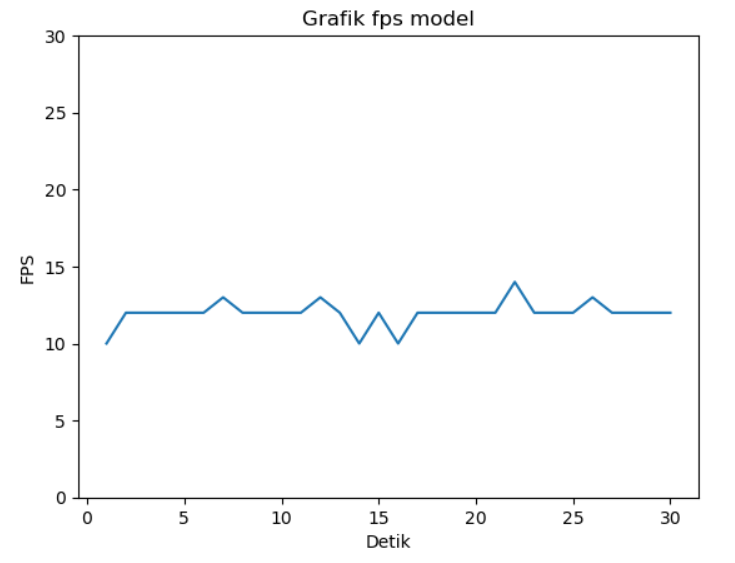
\includegraphics[scale=0.8]{gambar/pengujian-fps/grafik-pengujian-fps-vgg16.png}
  \caption{Grafik Pengujian \emph{Frame Rate} Model VGG 16}
  \label{fig:Grafik Pengujian Frame Rate Model VGG 16}
\end{figure}

\subsection{Pengujian Menggunakan Model MobileNet}
\label{subsec:Pengujian Menggunakan Model MobileNet}

MobileNets merupakan salah satu CNN yang seperti namanya, dapat digunakan pada perangkat mobile. Peneliti dari Google telah menciptakan arsitektur CNN yang dapat mengatasi kebutuhan resource komputasi yang berlebihan. Perbedaan mendasar antara arsitektur MobileNet dengan arsitektur CNN biasanya adalah penggunaan layer atau lapisan konvolusional dengan ketebalan filter yang sesuai dengan ketebalan citra masukan. MobileNet membagi konvolusi menjadi \emph{depthwise convolution} dan \emph{pointwise convolution}.

\begin{longtable}[!htb]{|M{25mm}|M{30mm}|M{30mm}|M{30mm}|c|}
  \caption{Hasil Pengujian Menggunakan Model MobileNet}
  \label{tb:Hasil Pengujian Menggunakan Model MobileNet}\\
  \hline
  \textbf{Variasi Pengujian} & \textbf{Total Data untuk Testing} & \textbf{Data Terprediksi Benar} & \textbf{Data Terprediksi Salah} & \textbf{Akurasi(\%)} \\ 
  \hline
  \endhead
  Pengujian Jarak 40 cm & 200 & 192 & 8 & 96 \\ \hline
  Pengujian Jarak 60 cm & 200 & 200 & 0 & 100 \\ \hline
  Pengujian Jarak 80 cm & 200 & 200 & 0 & 100 \\ \hline
  Pengujian Jarak 100 cm & 200 & 200 & 0 & 100 \\ \hline
  Pengujian Cahaya Terang & 200 & 193 & 7 & 96.5 \\ \hline
  Pengujian Cahaya Redup & 200 & 193 & 7 & 96.5 \\ \hline
  Pengujian Cahaya Gelap & 200 & 192 & 8 & 96 \\ \hline
  Pengujian Menggunakan Tangan Responden 1 & 200 & 199 & 1 & 99.5 \\ \hline
  Pengujian Menggunakan Tangan Responden 2 & 200 & 180 & 20 & 90 \\ \hline
  Pengujian Menggunakan Tangan Responden 3 & 200 & 191 & 9 & 95.5 \\ \hline
  Pengujian Menggunakan Tangan Responden 4 & 200 & 198 & 2 & 99 \\ \hline
\end{longtable}

Pada pengujian jarak, model mobileNet memiliki akurasi paling tinggi dibanding model yang lain. Berdasarkan Tabel \ref{tb:Hasil Pengujian Menggunakan Model MobileNet}, hasil akurasi rata-ratanya sebesar 99\%, dimana akurasi tertingginya ada pada angka 100\% dan terendahnya 96\%. Hasil ini tentu lebih besar dibandingkan dengan model yang penulis buat yang rata-rata akurasi jaraknya sebesar 97.5\%.

Dalam pengujian cahaya, akurasi model ini juga masih menjadi yang tertinggi dibandingkan model yang lain. Model ini dapat memprediksi secara stabil dengan tingkat akurasi selalu berada pada kisaran 96,5\%. Bahkan dalam kondisi paling gelap sekalipun tidak terjadi penurunan yang signifikan. 

Pengujian yang terakhir yaitu menggunakan variasi dari tangan responden, didapatkan hasil yang juga tertinggi diantara model lain. Rata-rata akurasinya diangka 96\%, dengan nilai akurasi paling kecilnya masih diangka 90\%.

\begin{figure}[!htb]
  \centering
  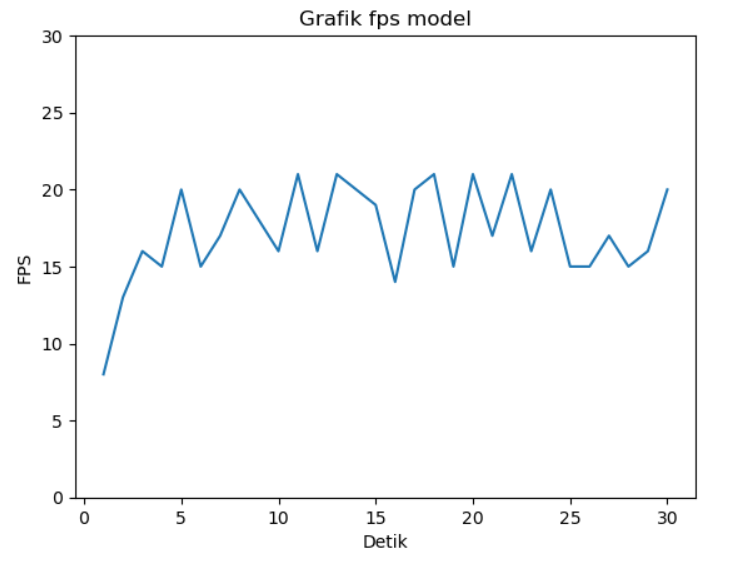
\includegraphics[scale=0.8]{gambar/pengujian-fps/grafik-pengujian-fps-mobilenet.png}
  \caption{Grafik Pengujian \emph{Frame Rate} Model \emph{MobileNet}}
  \label{fig:Grafik Pengujian Frame Rate Model MobileNet}
\end{figure}

Sedangkan, dalam pengujian \emph{frame rate}, model \emph{MobileNet} ini masih lebih tinggi dibandingkan model \emph{Resnet50} maupun \emph{VGG 16}. Dapat dilihat dalam grafik Gambar \ref{fig:Grafik Pengujian Frame Rate Model MobileNet}, rata-rata yang dihasilkan sebesar 17.26 FPS. Namun, FPS dari model ini masih lebih kecil dibandingkan model yang dibuat oleh penulis. Karena memang dari sisi jumlah layer dan hasil akhir ukuran file model jauh lebih kecil. Pada model \emph{MobileNet} ukuran file modelnya sebesar 136 MB. Sedangkan model yang dibuat penulis ukuran filenya hanya sebesar 43 MB saja.

Berdasarkan penyajian data dan analisa ini dapat dikatakan bahwa model \emph{MobileNet} memiliki performa yang paling baik diantara semua model yang diuji pada tugas akhir ini. Tingkat akurasi yang dihasilkan baik pada kondisi yang ideal maupun kurang ideal, model ini masih menghasilkan semua akurasi diangka lebih besar dari 90\% semuanya. FPS yang dihasilkan juga lebih tinggi dibanding model \emph{Resnet50} dan \emph{VGG 16} dengan angka 17,26 FPS.

\subsection{Pengujian \emph{User Experience}}
\label{subsec:Pengujian User Experience} 

Skenario pengujian yang terakhir adalah pengujian \emph{user experience} dimana dalam pengujian ini terdapat beberapa responden yang diminta untuk mencoba program yang dibuat. Mereka kemudian diminta untuk menjawab beberapa pertanyaan mengenai seberapa baik pengalaman penggunaan mereka dalam bentuk kuesioner. Melalui data tersebut dapat menguji apakah program ini dapat lebih baik dibandingkan dengan cara kontrol presentasi lain yang sudah tersedia saat ini.

\subsubsection{Model Kuesioner yang Digunakan}
\label{subsubsec:Model Kuesioner yang Digunakan}
Terdapat beberapa cara dalam menguji \emph{user experience}, Salah satunya dengan \emph{User Experience Questionare} (UEQ). UEQ berisi kuesioner yang mudah serta efisien, dan berguna untuk mengukur \emph{user experience} pada sebuah produk yang interaktif. \emph{User Experience} disini didefinisikan sebagai persepsi dan tanggapan seseorang yang dihasilkan saat suatu produk tersebut digunakan. Dengan demikian, \emph{User Experience} dipandang sebagai konsep yang mencakup semua jenis reaksi emosional, kognitif atau fisik mengenai produk jadi yang konkret atau bahkan hanya produk yang masih diasumsikan pembuatannya. Penilaian penggunaan produk ini dapat dinilai baik saat sebelum, selama dan setelah digunakan \parencite{AndreasHinderks}. 

UEQ mengukur menggunakan kuesioner yang berisi skala dan mencakup kesan komprehensif tentang (\emph{User Experience}). Terdapat enam skala penilaian akhir dalam UEQ, berikut rinciannya.

\begin{enumerate}[nolistsep]
  \item\emph{Attractiveness}. \emph{Attractiveness} atau daya tarik menilai kesan secara keseluruhan dari suatu produk. Penilaian ini mengukur apakah pengguna cenderung menyukai atau tidak menyukai produk yang diuji. Oleh karenanya, produk harus dibuat untuk terlihat menarik, menyenangkan, ramah pengguna dan menyenangkan. 
  \item\emph{Perspicuity}. \emph{Perspicuity} atau kejelasan adalah bagian yang menilai seberapa mudah produk untuk dikenali dan dipelajari cara penggunaannya. Sehingga produk harus dibuat untuk bisa melakukan tugas tertentu dengan cepat, efisien, dan dengan cara yang pragmatis.
  \item\emph{Efficiency}. \emph{Efficiency} merupakan penilaian yang mengukur apakah pengguna bisa menyelesaikan fungsi atau fitur tertentu dengan melalui usaha yang sedikit mungkin. Selain itu, reaksi dari produk apakah dapat bereaksi dengan cepat atau tidak. Karena itu, produk harus sederhana, dan mudah dipelajari.
  \item\emph{Dependability}. \emph{Dependability} atau ketepatan menilai apakah interaksi dengan produk ada dibawah kendali dari pengguna. Penilaian ini berkaitan dengan tingkat keakuratan sehingga interaksi yang dihasilkan sesuai dengan prediksi dari pengguna. Hal ini juga berhubungan dengan tingkat keamanan yang dihasilkan dari produk, karena apabila output yang terjadi tidak sesuai dengan yang diharapkan, dapat menimbulkan kesalahan prediksi yang tidak dapat diantisipasi oleh pengguna . Sehingga, item ini menilai apakah produk dapat diprediksi, aman, dan memenuhi harapan pengguna atau tidak.
  \item\emph{Stimulation}. \emph{Stimulation} adalah bagian penilaian yang dapat memiliki efek rangsangan perasaan positif. Perasaan yang timbul ini bisa perasaan menarik, menyenangkan, memotivasi, ataupun seru saat menggunakan produk. Oleh karena itu, produk harus dirancang sedemikian rupa hingga dapat menimbulkan efek rangsangan perasaan menarik dan menyenangkan.
  \item\emph{Novelty}. \emph{Novelty} atau kebaruan merupakan bagian pengukuran yang menilai seberapakah kreatif dan inovatifnya suatu produk. Apabila suatu produk itu memilki nilai inovasi dan kreatif didalamnya, tentu dapat menimbulkan kesan menarik minat bagi pengguna. Sehingga, produk harus memiliki ide awal yang dirancang secara inovatif dan kreatif, serta menggunakan teknologi yang sesuai dengan perkembangan zaman.
\end{enumerate}

\begin{figure}[!htb]
  \centering
  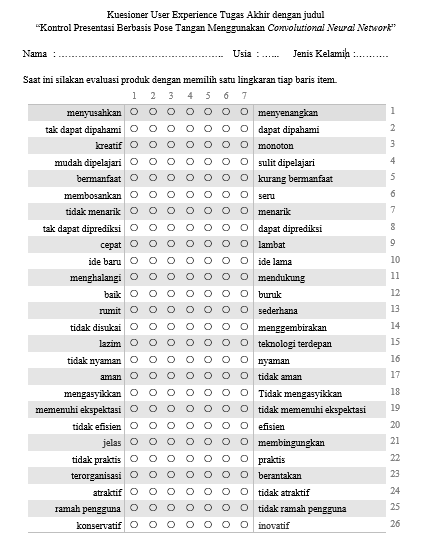
\includegraphics[scale=1.5]{gambar/pengujian-user-experience/soal-kuesioner.png}
  \caption{Soal Kuesioner}
  \label{fig:Soal Kuesioner}
\end{figure}

Pertanyaan yang ada pada kuesioner ini berjumlah 26 item. Setiap item ini menunjukkan skala satu sampai tujuh, dimana penilaian positifnya ini tergantung pada letak item tiap nomor soalnya. Sebagai contoh, dapat dilihat pada gambar \ref{fig:Soal Kuesioner} dimana pada item nomor satu menyenangkan ada pada sisi kanan. Sehingga, semakin skalanya kearah kanan, maka semakin positif penilaiannya. Namun, pada soal nomor tiga, penilaian kreatif ada pada sisi kiri. Hal ini membuat penilaian positifnya justru ada pada skala yang semakin kecil. 

Tujuan dari dibuatnya pertanyaan seperti ini, agar pengguna yang mengisi kuesioner bisa dapat menilai lebih objektif dan teliti. Apabila penilaian positifnya semuanya ada pada sisi kanan, dikhawatirkan beberapa responden tidak melihat item pada tiap soalnya dan hanya mengisi di sisi yang positif semua atau negatif semua.  

Berdasarkan pertanyaan dalam tiap item kuesioner, dikumpulkan dan dianalisis penilaiannya seperti apa. Dalam penggunaan UEQ, sudah terdapat \emph{tools} yang dapat digunakan untuk menilai output dari pengujian ini. Outputnya berupa diagram yang dengan nilai tertentu dari setiap enam skala penilaian dalam UEQ yaitu daya tarik, kejelasan, efisiensi, ketepatan, stimulasi, dan kebaruan.

\subsubsection{Distribusi Responden}
\label{subsubsec:Distribusi Responden}

Pengambilan data kuesioner dilakuakan pada area kampus, dimana umumnya responden memiliki latar belakang sebagai pelajar atau mahasiswa. Alasan pengambilan responden dengan latar belakang tersebut karena mereka adalah salah satu bagian masyarakat yang paling sering melakukan kegiatan presentasi. Sehingga, sasaran responden dianggap tepat dalam pengujian kali ini. 

Jika dilihat berdasarkan usia, responden yang mengisi kuesioner berada pada rentang usia antara 21 sampai 22 tahun. Sedangkan berdasarkan jenis kelamin didominasi oleh pria dengan rincian 86\% pria dan 14\% wanita seperti yang terlihat pada Gambar \ref{fig:Persebaran Data Gender}  

\begin{figure}[!htb]
  \centering
  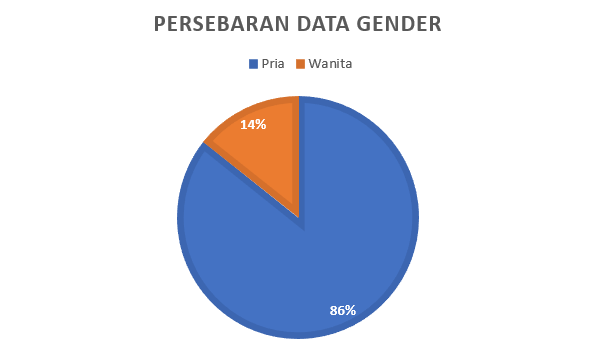
\includegraphics[scale=1]{gambar/pengujian-user-experience/persebaran-data-gender.png}
  \caption{Persebaran Data Gender}
  \label{fig:Persebaran Data Gender}
\end{figure}

\subsubsection{Hasil Analisa Kuesioner}
\label{subsubsec:Hasil Analisa Kuesioner}

Berdasarkan pengumpulan kuesioner dari responden yang disebutkan pada \ref{subsubsec:Distribusi Responden}, data dimasukkan kedalam \emph{'tool'} yang disediakan dari metode UEQ. Output yang dihasilkan \emph{'tool'} ini berupa data grafis yang menunjukkan seberapa positif atau negatif evaluasi yang diberikan oleh responden. 

Nilai untuk satu item digambarkan dalam skala antara 1 sampai 3. Nilai antara -0,8 dan 0,8 mewakili evaluasi yang kurang lebih dianggap netral. Sedangkan, nilai lebih dari 0,8 mewakili evaluasi atau penilaian yang positif. Sebaliknya, nilai kurang dari -0,8 mewakili evaluasi atau penilaian negatif. Jadi, apabila hasil penilaian ada pada kisaran skala antara -3 berarti sangat buruk dan +3 berarti sangat baik. 

\emph{Ouput} dari grafis yang pertama adalah terkait dengan rata-rata jawaban responden pada setiap item soal. Seperti yang tertera pada Gambar \ref{fig:Jawaban Rata-rata Setiap Item Soal}, rata-rata jawaban dari responden memberikan penilaian yang bersifat positif karena nilainya lebih besar dari 0,8. Terdapat beberapa item penilaian yang dinilai paling positif yaitu item kemudahan untuk dapat dipahami, baiknya program, keamanan saat digunakan, dan kepraktisan penggunaan. 

\begin{figure}[!htb]
  \centering
  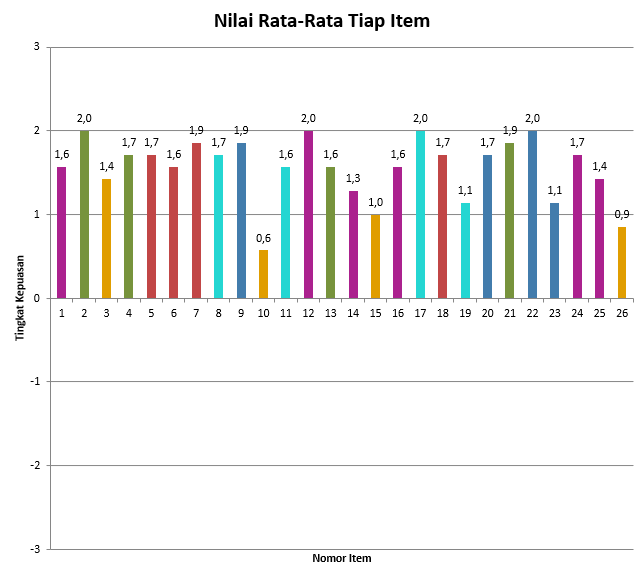
\includegraphics[scale=1.15]{gambar/pengujian-user-experience/rata2-tiap-jawaban.png}
  \caption{Jawaban Rata-rata Setiap Item Soal}
  \label{fig:Jawaban Rata-rata Setiap Item Soal}
\end{figure}

Namun, terdapat penilaian yang terhitung bukan positif namun masih ada pada rentang netral. Penilaian itu terkait dengan item daya cipta dan inovasi. Maksud dari item ini adalah terkait dengan seberapa inovatif dan baru ide dari topik tugas akhir ini. Berdasarkan penilaian ini dapat dinyatakan bahwa inovasi dan ide dari tugas akhir ini memang bukan sesuatu yang sangat baru, namun tidak dapat dinyatakan tertinggal juga. 

Berdasarkan semua item soal dalam kuesioner, dapat dikelompokkan menjadi enam penilaian utama yang disebutkan pada \ref{subsubsec:Model Kuesioner yang Digunakan} yaitu \emph{Attractiveness, Perspicuity, Efficiency, Dependability, Stimulation, dan Novelty}. Hasilnya dapat dilihat pada Gambar \ref{fig:Hasil Penilaian User Experience}. 

Pada penilaian pertama terdapat \emph{Attractiveness} atau daya tarik yang mendapatkan poin 1,595. Hal ini menunjukkan bahwa program yang dibuat dapat dinilai terlihat menarik, menyenangkan, serta ramah untuk pengguna yang baru mencoba.

Penilaian yang kedua adalah \emph{Perspicuity} atau kejelasan, dimana didapatkan poin sebesar 1,786. Nilai tersebut menunjukkan bahwa program bisa melakukan tugasnya dengan cepat, efisien, dan dengan cara yang pragmatis.

Penilaian yang ketiga adalah \emph{Efficiency}. Poin yang didapatkan untuk efisiensi sebesar 1,679 yang berarti pengguna bisa menggunakan suatu fungsi atau fitur tertentu dengan melalui usaha yang seminimal mungkin.

Item penilaian yang keempat disebut sebagai\emph{Dependability} atau ketepatan. Didapatkan nilai poin 1,607 yang berarti nilai tersebut menunjukkan bahwa interaksi antara pengguna dengan program yang dijalankan masih ada dibawah kendali dan sesuai dengan perkiraan atau harapan pemakainya.
  
Dalam item penilaian yang kelima ada \emph{Stimulation}. Poin yang didapatkan sebesar 1,714. Hasil penilaian ini menunjukkan bahwa pengguna mendapatkan efek rangsangan perasaan yang positif, baik itu perasaan menarik, menyenangkan, dan seru.

Item Penilaian yang terakhir adalah \emph{Novelty} atau kebaruan. Dalam item penilaian ini didapatkan poin sebesar 0,964. Memang angka ini tidak terhitung cukup tinggi dibandingkan dengan penilaian sebelumnya, namun masih termasuk dalam rentang penilaian positif. Oleh karenanya, program ini masih bisa dikatakan sebagai produk kreatif dan inovatifnya, walaupun memang dinilai oleh beberapa pengguna bukan sebagai suatu ide yang benar-benar baru.

\begin{figure}[!htb]
  \centering
  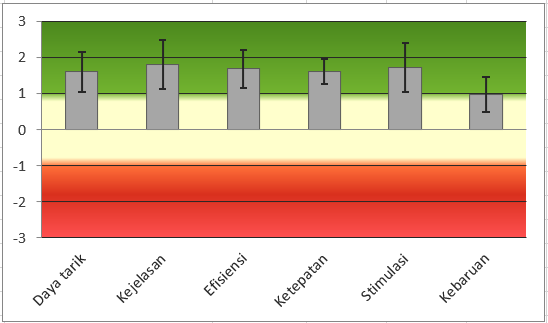
\includegraphics[scale=1.1]{gambar/pengujian-user-experience/hasil-tiap-penilaian.png}
  \caption{Hasil Penilaian \emph{User Experience}}
  \label{fig:Hasil Penilaian User Experience}
\end{figure}

Berdasarkan analisa pada pengujian \emph{user experience} dapat diambil penilaian bahwa program yang dicoba memberikan pengalaman pengguna dengan hasil reaksi evaluasi yang bersifat positif, terutama dari aspek kemudahan untuk dipahami, kepraktisan dalam penggunaan, dan memberikan pengalaman perasaan menarik dan menyenangkan.